\chapter{Model}  \label{chapter-model}
\epigraph{One of the very important components in the urban and agricultural land use model is the so-called \gls{bid-rent curve}. Regional and urban economists, city planners, and economic geographers have used this curve extensively as an analytical device.}{Yeung-Nan Shieh \cite{shiehWilhelmLaunhardtBidRent2004}}

% FUTURE WORK Because our goal is to extend the current model by introducing speculative motives and financialization, we retain the single-type household of the basic model, we defer the question of the differential effect on household types for later work.  

%because a key feature of this model is that it formally captures how finalization works to capture the 
%financialization is aimed at capturing the 
%rents generated by growth and specifically urban growth..

% LINK WHAT TO WHAT..
% The feature of the model that provides the necessary link is known as the `\gls{bid-rent curve}.' We will incorporate the financial sector into the land market using the bid-rent curve.

%We begin in Section~\ref{section-financialize} with a definition of the act of financializing transactions and markets,  and discuss some significant examples. 

%Finally, in  Section~\ref{section-system} we explain how financialization might affect the housing market as a system and some consequences for society in general. 
%At that point we can introduce our specific hypotheses and how we intend to test them.
% We focused on modeling the effects of financialization on and through the urban housing market to \textbf{WHY?}. 
% This is where the ghttps://www.facebook.com/profile.php?id=100000594429550eneral process of financialization At that point we can introduce our specific hypotheses and how we intend to test them.
% We therefore begin with a narrow and strict definition of the act of finacializing, followed by an explanation and examples. We then go on to explain how the term is applied at the level of systems and while markets.
% At that point we can introduce our specific hypotheses and how we intend to test them.

% COULD CALL THIS THEORETICAL DEVELOPMENT OF THE MODEL AND MAKE A SEPERATE IMPLEMENTATION CHAPTER

% This chapter describes the specific formulations % (**E USE A MORE SPECIFIC WORD THAN LINKS) % #E BUILD A PCITURE OF HOW THE MODEL DRAWS THESE TOGETHER \dots LIKE IT TAKES THESE THREAD (LIST THEM) AND COMBINES THEM INTO A MODEL THAT EXPLORE \dots USE THIS PARRARAPH TO DESCRIBE THE EXACT INTERCONNECTIONS

% the theoretical discussions of the previous chapters with an agent-based simulation model. 

% At the heart of the model is a real estate mark et in which owners, tenants, new entrants to the city and non-resident investors participate. To do that we build up our model in a series of steps beginning with a notion of economic value, adding potential speculative gains, and finally describing a transaction process. %We need to specify the market process in more detail. (???) % i DONT UNDERSTAND IF YOU ARE SAYING YOU NEED THIS? THE MODEL FILLS THIS GAP?? OR THIS IS AFILLER SENTECEN??? 

% This chapter introduce the urban spatial model and labour supply, models the production function with urban scaling of agglomeration effects with density, then introduces a model of financial investment/speculation into a spatially explicit land market model, then calculates profit, considers who gets the profit, and draws conclusions. 



%     MOVE THIS?
%Recent urban models %, on the other hand, tend to focus on the locational implications of land and transportation costs on the location of people. Wealth distribution is  often ignored. 

% - need to  model production, specifically the rising production with density. 
%There is an extensive formal apparatus in economics for considering the relation of production and output. 

% \section{The general structure of the model}
In this thesis  we describe an agent-based spatial model of an urban housing market that includes a production function modelling how urban regions generate wealth and an explicitly financialized housing market.  Where previous chapters %***E EDIT: DISCUSSED IN GENERAL THE PRINCIPLES OR DISCUSSED THE ENERAL PRONICPLES 
discussed the general principles that underlie our theoretical model, this chapter presents details about the how the variables in the computational model are defined. %Where, for example, we talk about expected price in Chapter~\ref{ch_financialization}, here we  provide the formula we use in our simulations.

% The model is introduced in the following sections:
% \begin{enumerate}
% \item In Section~\ref{sec_model_blocks} we  begin by describing the major blocks of the model. 

% \item In Section~\ref{sec_model_dynamics}  we make some comments on the dynamic properties of the model we have constructed. 

% \item In Section~\ref{sec_model_variables} we describe how a series of key  variables are constructed. The variables enter the decision-making process of agents in the market. 

% \item In Section~\ref{sec_model_bid_price}     

% \item In Section~\ref{sec_model_bargaining}    

% \item The treatment of time a periods and discounting is discussed in Section~\ref{sec_model_time}. 
%  Section~\ref{sec_model_price_expectataions}


% \item In Subsection~\ref{sec:Production-fn} we introduce the production function, introduce the labour supply and the urban model, the source of the surplus,  then we calculate profit, consider who gets the profit, and from there we draw our conclusions.. then we calculate the urban surplus, and consider who gets it. 

% \item Appendix~\ref{appendix-model-implementation} gives more details, describing the calculations, and showing how the model is implemented in code. 

% \end{enumerate}

% % % In subsequent sections  .. (Derivation details in Section~\ref{section-derivations})


% \section{The three major blocks of the model}\label{sec_model_blocks}

Our goal has been to make an accessible model % model as accessible as the \Gls{Alonzo model} 
that can provide insights about the impact of the financialization of the housing market on urban productivity and wealth distribution.  The  model has three major blocks:

{\newpage\thispagestyle{empty}
\vspace{-1.5cm}
\begin{figure}
\vspace{-1cm}
\begin{adjustwidth}{-0.24\textwidth}{-0.24\textwidth}
\centering
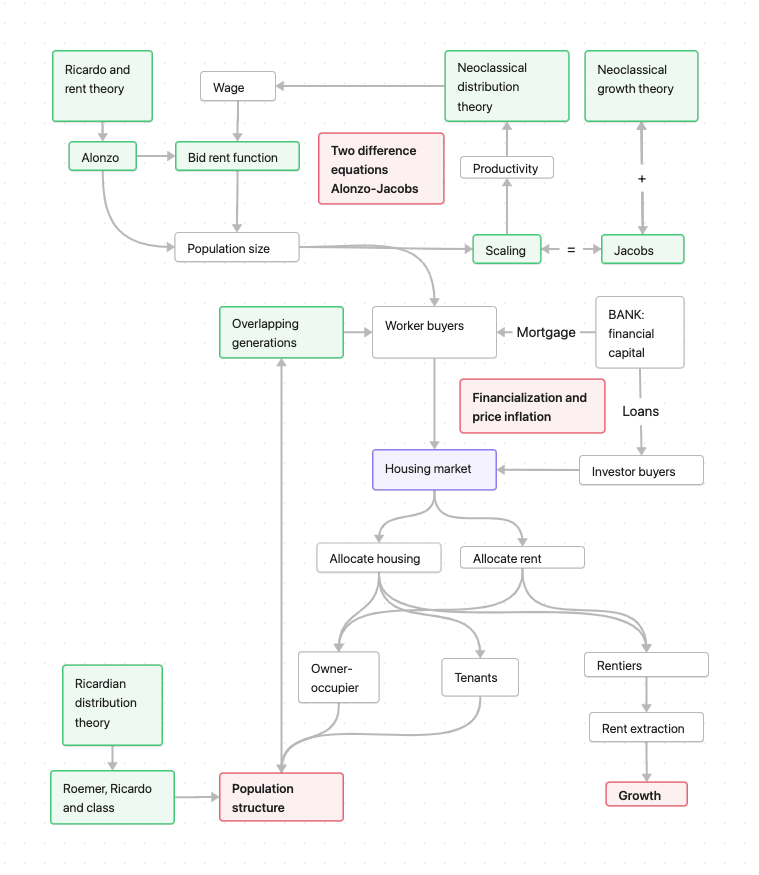
\includegraphics[scale=.6]{fig/flow-full-model.png}
\label{Stylized model flow.}
%\pagestyle{headings}
% \usetikzlibrary{positioning}
%\begin{tikzpicture}[remember picture,overlay,shift={(current page.north east)}] \node[anchor=north east,xshift=-1cm,yshift=-1cm]{\includegraphics[width=1cm]{example-image-a}};\end{tikzpicture}
\end{adjustwidth}
\caption{Model logic }\label{fig-flow-full-model}
\end{figure}
}

\begin{enumerate}
\item We incorporate the spatial structure of the city and its transportation system using a version of the \gls{bid-rent function} that drives all Alonso-style models. This equation is embedded in the decision of every agent because it determines the economic rent for each piece of property.

\item We incorporate the fundamental wealth production process of the city using an \gls{urban scaling} law that captures Jacobs-style agglomeration effects. This allows us to bypass the complexities of labour and goods market adjustments and instead to deal with the underlying long-term relationship between city population and production. We call the combination of this Jacob agglomeration effect with the Alonso model an \gls{Alonso-Jacobs model}. Our \gls{agent-based model}, in effect, mimics two difference equations, operating on two aggregate variables, and incorporating the major insight of a half-century of \gls{neoclassical growth theory}.

\item To link the Alonso-Jacobs model to the financial system, we develop an \gls{overlapping generations} model of the housing market with borrowers and lenders that tracks ownership and wealth. This turns out to be the most detailed and computationally-intensive part of the model. To model the effects financializing housing in our \gls{agent-based model} we are forced to carefully specify the microeconomics of individual decisions. % In Section~\ref{section-micro},
We therefore, we describe the microeconomic objective function that individuals and our bank agent employ in deciding to purchase a property. 
\end{enumerate}
In addition to the main blocks, to explore the potential effect of financialization on urban productivity 
\begin{quotation}\noindent We introduce an investment link from housing ownership to the urban production firm's production function.
\end{quotation}




Figure~\ref{fig-flow-full-model} shows the model logic.  The following three sections will discuss each of the three primary components, the spatial structure, the productivity mechanism, and the housing market in order.  To focus the model on the core questions of the relationship between urban productivity and rent, we keep the first two components,  the spatial structure and the growth mechanism,  as simple as possible, modeling the market for housing in more detail. 

% ANALYSIS???Finally, in  Section~\ref{section-system} we explain how financialization might affect the housing market as a system and some consequences for society in general. %At that point we can introduce our specific hypotheses and how we intend to test them.

\section{Spatial structure}

% In this section, we introduce the basic structure of the model, drawing on the circular city model.  
%  
% We build a spatially explicit agent model where agents work in one location and incur costs travelling to work. This work integrates a model of production and labour into a standard spatial model of the city. In this section, we introduce an analytic model of production and a labour market in a stylized circular city. 

% \subsection{Labour supply for production}
We begin with a model of a circular city.\footnote{In our computational model we use a grid structure with  a block metric, which is computationally more convenient and provides a slightly more natural representation of the property structure of actual cities.} %- INTRO CITY/APPROACH?
In the \gls{Alonso model} \cite{alonsoTheoryUrbanLand1960, alonsoLocationLandUse1964}, firms are located at the centre of a circular city, the central business district. Residents live distributed across space, can take jobs, and commute to work at the urban center. 
% In the simplest version, firms concentrate at the city centre. Workers are spread over space and pay transportation costs to commute.



Firms produce perfectly \gls{substitutable} % For simplicity, firms produce a variety of
goods that they sell into a commodity market. Demand for the \gls{product} is \gls{perfectly elastic}, so the price remains constant. 
Firms purchase the time of workers. %to capture the product of their effective labour
%and enjoy the product of \gls{effective labour} . They can produce more goods by hiring additional workers. 
With the neoclassical model of distribution,\footnote{Clark's neoclassical assumption is that workers receive the value of their marginal product \cite{clarkDistributionWealthTheory1899}.} 
% We assume that the neoclassical model of distribution holds in the long run and 
workers receive the value of their marginal product. 
Because of agglomeration effects, workers in the city are more productive than workers in the countryside. They therefore receive an \gls{urban wage premium}.

% TODO this shows the dynamics of a local economy, trade dynamics dominate local dynamics in many cases, that is explored with the addition of more cities and centres. 
%NEED TO INTRODUCE SUBSISTENCE WAGE BEFORE MENTIONING IT ABOVE %[MAYBE This follows xyz's approach, and makes it possible to explore resident's choice to work]. 

As in the Alonso model, described in Chapter~\ref{chapter-space}. The \gls{urban wage premium} and transportation costs together determine both the radius of the circular city and the size of the labour force, %?There is no fixed boundary and the size of the city is determined by the utility that can be achieved in competing regions of competing for labour.
% and as in the standard circular city model the constraint on growth is provided by transportation costs, which limit the size of the commuter-shed and therefore the labour force at any wage. 
 %The raidus of the commuter shed is thus,  %The farthest workers will travel to work is thus 
% The  productivity of the city attracts people. 
since agents work if the wage premium is greater than the cost of travel. % Living close to work has value to workers because it saves the cost of transportation. 
The higher the wage, the farther workers will commute. %This is the core of the Alozo circular city model.
The farthest that workers will travel is $\frac{w}{{c}}$, where ${c}$ is the cost of transportation per unit distance. This defines the radius of the city and the commuter shed.

The \gls{urban labour supply} is an \gls{aggregate} measure that emerges from individual agents' choice to commute. Considering a standard, Alonzo-style \gls{circular city} with a uniform lot size, $s$, and  one worker per unit land. For illustrative purposes, the labour available is simply the area of the circle divided by the lot size 
\begin{equation}
%=  \frac{\pi}{s}(c^{max})^2	
 N = \frac{\pi}{s} \left(\frac{w}{{c}}\right)^2,
%   =\frac{\pi}{{c}^2 s} w^2,
\label{eqn-labour-supply1}
\end{equation}
where $\omega$ is the wage premium, $c$ is the cost of transportation, and $s$ is lot size (land per person).\footnote{The formula is for the case with a uniform density of one worker per lot. In the computation model density is a variable.} This is the equilibrium \gls{urban labour supply} function for the circular city. For a city with an idealized rectangular grid of streets, the city shape is rectangular rather than circular and the labour supply function is \[N= \frac{2}{s}\left(\frac{w}{{c}}\right)^2.\] %which is a \cite{GET_migration_equilibOR_pop_equilib_condition}. %It defines the quantity of labour available.

%\footnote{See the discussion of model extensions in Appendix~\ref{appendix-future-work}.}.
% To get the \gls{urban wage premium}, we can write the inverse of the labour supply function:
% \begin{equation}
% w= (\frac{ {c}^2s}{\pi})^{0.5} L^{0.5}.
% \label{eqn-inverse-labour-supply}
% \end{equation}

\section{Agglomeration and productivity}\label{sec:Production-fn}


% *** ADD BACK? To study the productivity of cities, we incorporate Jacobs-style agglomeration economies (\cite{beaudryWhoRightMarshall2009, vanderpanneAgglomerationExternalitiesMarshall2004, jacobsEconomyCities1969}), using an approach similar to the way the \gls{Solow-Swan model} incorporates labour-augmenting technical change with a \gls{Cobb-Douglas} production function, and building the production function into a standard Alonso-style model of an urban economy.
%, using a simple Cobb-Douglas production function. 
% We incorporate the estimated scaling relationship in 
%The scaling result at the level of the city allows us to incorporate the agglomeration effect in a \gls{circular city} model, 
The agglomeration effect that augments the productivity of workers means firms produce more goods with a given stock of labour if the city is larger and urban workers are more productive. Figure~\ref{fig-agglomeration-surplus} in Chapter~\ref{chapter-growth} illustrates the increasing returns to urban size. % than rural workers due to the positive agglomeration externalities. 
These increasing returns mean that urban firms can %Urban firms can therefore 
pay a premium that depends on, among other things,  the size of the city. Because workers face transportation costs, firms have to pay this premium to attract workers. % , above the subsistence wage.
%in a city with more people, as introduced in Chapter~\ref{chapter-growth} on growth.(**E SEE NOTE HERE) % #E i THINK YOU NEED TO FLESH THIS OUT, i'M NOT SURE EXACTLY WHAT YOU ARE SAYING. JUST BE A BIT MORE SPECIFIC AND FLESH OUT. 
% \subsection{Labour force}
%There are also firms that produce goods to sell. (???) % #E HOW IS THIS DIFFERENT THAN THE FIRMS PRODUCING GOODS IN THE PREVIOUS PARAGRAPH???

% Firms sell the goods they produce into a commodity market. 
 %, which are both exported and locally consumed 
% to sell into a large market, at a fixed price. 





To focus the model on urban productivity and the growing urban wage premium, we model workers as receiving a \gls{subsistence wage} $\psi$ in the countryside.\footnote{Classical economists employed the \gls{subsistence wage} assumption to simplify their analysis in a similar way.} % 
%\cite{GET_classical-subsistence-wage}.
%
% CLASSICAL POLITICAL ECONOMY, THE SUBSISTENCE ...
% American Economic Association
% https://www.aeaweb.org › conference › retrieve
% PDF he Classical Understanding of the Subsistence Wage. While the historical run of classical political economy runs from William Petty through David.
This subsistence wage could come from work in the local community, living off the land, family support, social support, or something else. 
 % The model is set up so that all of an urban  tenant's  income is spent on  basic living costs, $\omega$, transportation $td$ or rent. Disposable income for owner occupier $i$ is therefore just the return  $\omega -dc$ which may accumulate as a financial asset.
% To attract workers to live in the city and commute to the central business district, firms pay the  \gls{urban wage premium}, $\omega$, in addition to  the subsistence wage $\psi$. 
%\footnote{See parameter appendix Section~\ref{section-wage-premium} for a discussion of the empirical literature on the \gls{urban wage premium}.}. 
% When workers take a job, they give up the subsistence income and, % instead receive a wage from their employer. % When workers take a job, they  receive, in addition to the subsistence wage,  the wage premium  from their employer. 
Urban workers give up the subsistence income and receive the \gls{urban wage}, $\psi +  \omega$, the subsistence wage plus the \gls{urban wage premium} that firms pay to attract workers. 
% When we assume an subsistence wage with a specific share  applied to housing we are implicitly assuming that landlords are seeking to claim the value of the rents. It makes it possible to explore whether and how tenants and even owners may be squeezed towards a \gls{subsistence frontier}. %whatever value the can. % tenants are squeezed by landlords. % DOES THE 'THIS' REFER TO THE FORMALIZATION OF WARRANTED RENTS?

\subsection{Wage determination}

According to \gls{neoclassical distribution theory}, the firm maximizes profit by setting the marginal value of the product of each \gls{factor of production} equal to the unit cost per factor.\footnote{Appendix~\ref{appendix-firm-theory} has more detail on the theory of the firm underlying the treatment here.} If we calculate the physical marginal product of labour for the Cobb-Douglas with the Jacobs externality $A(L^T)$ from Equation~\ref{eqn-production-jacobs}, we get 
\begin{align}\label{eqn-model-MPL}
y              =&  A(L^T) k^\alpha n^\beta \nonumber\\ 
\die{y}{L}     =&\beta A(L^T) k(t)^\alpha n^{\beta-1} \nonumber\\
                =&\frac{\beta A(L^T) k(t)^\alpha n^\beta}{n} \nonumber\\
                =& \frac{\beta y}{n}.
\end{align}
This is clearly positive and increasing in $L^T$, the aggregate labour force for the city.  It follows that population growth increases marginal product in this model. 


Since optimizing firms are assumed to adjust their wage offer and hiring to achieve a wage that is equal to the  marginal \textbf{value} product of labour 
\begin{align}\label{eqn-model-MPL-w}
             \omega + \psi   =& P_y\frac{\beta y}{n}.
\end{align}
where $P_y$ is the price of output. We assume the price of output is constant and will treat it as \$1 per unit output for the rest of the chapter. As a result, the wage increases, perhaps with a lag, when urban population  rises 
\begin{equation}
 \die{(\omega + \psi)}{L^T} >0.
\label{eqn-wage-population}
\end{equation}
In our model the subsistence wage $\psi$ is fixed, so the wage premium must rise if the marginal product of labour rises.  We have shown that a rising wage premium increases the distance that workers will travel to work, so the city grows and population rises, as the upper loop in Figure~\ref{fig-flow-full-model} illustrates. 

 

Equation~\ref{eqn-model-MPL-w} is an equilibrium condition for the firm. Firms, however,  are agents setting wages and hiring while labour supply and demand are shifting.    We assume that they do know the marginal product of their current workforce and can observe the wage level from period to period. It is reasonable to assume that when their marginal product of labour rises they adjust both their labour demand and their wage offers. The marginal product of labour can be seen as a target wage. Equation~\ref{eqn-model-MPL-w} implies that the firm's target labour demand is 
\begin{equation}
           n  = \frac{\beta y}{\omega + \psi}.
\label{eqn-labour-demand}
\end{equation}
We assume it is reasonable to assume $\omega$, and the wage, $n$, the size of the firm's workforce,\footnote{The analytic model offers an equilibrium solution with full employment. The assumption of full-employment is unrealistic. Workers are laid off, and take time to find new employment. The time people spend moving between jobs causes frictional unemployment which varies with economic conditions. Introducing a constant or ``natural'' rate of unemployment would introduce additional dynamics, however it would be unlikely to affect the results that interest us.} 
Both adjust slowly toward target values in each period. We also allow the number of firms to adjust gradually.\footnote{We have assumed that the firm does not notice that, by hiring, it increases the agglomeration effect for the city. This assumption is convenient as well as plausible since it removes a term , $\frac{F\gamma y}{N} =\frac{\gamma y}{n}$, that is both small very hard to observe.}


% The city has single firm facing a fixed price for output. 

% IS THIS DUPLICATION? I THINK THE Solow-Swan model IS INTRODUCED IN SPACE CHAPTER. MOVE THIS TO SPACE CHAPTER IF NEEDED?
% In the \gls{Solow-Swan model}:
% \begin{equation} 
% Y(t) = K(t)^{\alpha}(A(t)L(t))^{\beta}
% \label{eqn-solow-swann}
% \end{equation}
% where $Y$, $K$ and $L$ are aggregate output, capital, and labour, respectively,  $A$ is the term the Solow-Swan model introduced for technology. The technology term capture the growth of labour productivity over time, $\alpha$ is the \gls{elasticity} of output with respect to capital, $\beta$ the elasticity of \gls{output} with respect to \gls{effective labour}, and $t$ time. If $\beta=1-\alpha$, this is a \gls{constant returns to scale} \gls{CRS} production function at the firm level.
% In the Solow-Swan model all factors of production are fully employed, and initial values $A(0)$, $K(0)$, and $n( 0 )$ are given. The number of workers, i.e. labour, as well as the level of technology grows exogenously at rate %s are $n$ and it   $g$,% respectively:  $L(t)=L(0)e^{nt}$     $A(t)=A(0)e^{gn}$ 
% This model uses a similar functional form to look at the effect of population density increasing % productivity. %how density increases in in  % It models how population increases productivity. 


%%%%%.   MAYBE REINTRODUCE THIS
% The urban wage premium scales with the agglomeration effect. The \glspl{agglomeration effect} ensure urban \gls{output} is more than proportional to urban population: 
%  \begin{equation}
%  Y\propto N^{\beta},
%  \label{eqn-production-population}
%  \end{equation}
% where $\beta$ is the elasticity of output with respect to capital, $\beta > 1$ where the agglomeration effect is positive. % Setting $\beta = 1$ would be the \gls{constant returns to scale}. $\beta - 1$ is the extra return that comes from adding to people the city. That return is the agglomeration effect that belongs to the city, it could go to the people.

% We can put this together using a model of the production function. We implicitly use a three-factor model of \gls{production}, where production, is a function of capital and labour as well as a third factor, a Solow-Swan style term for labour augmenting technical change, with an \gls{agglomeration} effect, $A(N)$, in place of technology, $A(t)$. Output is:

%\subsection{aggregate urban output}
% \begin{equation}
% Y=A()K^{\alpha }(L^\beta}.
% \label{eqn-prod1}
% \end{equation}
% where $K$ is capital, $\alpha$ is the elasticity of output with respect to capital, $\alpha = \beta - 1$, and  $n$ is the \gls{urban labour supply}. $A(N)$ incorporates Jacob-style agglomeration externalities. $A(N)N$ is \gls{effective labour}.\footnote{The function  was discussed in Chapter~\ref{chapter-growth}.}

% \section{Agglomeration Appendix: Production Function}
% SORT APPENDIX/OTHER STUFF

% The agglomeration factor increases with population. It multiplies labour because agglomeration scales the productivity of workers.  
% It is a model of a productive urban economy since the centre is productive and demands labour.
% The growth of population feeds back into productivity. % We allow rising population to directly increase the wage.  
% We supplement the spatial model with agglomeration effects consistent with the literature. % in the base model. 
% There is an agglomeration effect, which
% The agglomeration effect means firms can also produce more goods by operating in a city with more people, because of the connections and interactions between people (CITE). 
 
 %, we assume the presence of scaling, consistent with neoclassical growth models as discussed in Chapter~\ref{chapter-growth}. 
%In this section, we introduce the basic structure of the production side and connect it to the literature on urban scaling. 
% We bypass the complexity of modelling firms, allowing population increases to directly increase urban wage premium.
%, It is straightforward to compute the rate of excess return for  this model. 

% We assume that the firm behaves as a price taker in the labour market as well, despite the fact that we model it as a \gls{monopsonist}\footnote{}. JUSTIFY/REPHRASE/EXPLAIN monopsonist. %ALSO DOES THIS GO HERE OR BELONG WITH PRIOR SECTION?

% Labour demand is thus a derived demand based on standard neoclassical theory with an equilibrium wage offer that is the marginal (value) product of labour for the firm. Specifically, hiring proceeds until the marginal product of labour is equal to the wage.

% The firm adjusts its labour force upward when the \gls{marginal product of labour} is greater than the wage by selecting from its list of job applicants.
% The firm adjusts its wage offer upward when the marginal product of labour is greater than the wage and it faces a labour shortage.  Labour shortage is a situation where the firm wants to hire but its list of job applicants is empty.

 %The marginal product of labour at the firm level is increasing in $L^T$, at a decreasing rate to ensure a labour market equilibrium exists for the model %, to connect with the analytic tradition of economic modelling by ensuring there is an equilibrium level of production.  
 
% If the marginal product increased, then a firm that got large enough would out-compete smaller firms, hire all labour, always be able to produce more wealth by hiring more people, and would always produce more wealth by hiring people than by firing people. This doesn't happen. 
% Perhaps, the firm hires employees who best fit its needs first, but to grow, eventually it must hire less selectively. Finding markets may get harder with growth. Perhaps expansion adds additional costs, building a parking lot, administration, acquiring a larger building. Whatever the explanation, the marginal product of labour declines. 




% labour adjustment costs include moving costs for the employee or hiring, firing, or training cost for the firm. (there might be a hiring, firing, or training cost on the firm side, or on the employee side: expected time to employment costs, moving costs, etc.)
%The assumption of monotonically declining  marginal product of labour is embedded in the production function, so it applies in the analytic and agent models.  Agglomeration effects can push the sum above one. When the exponents add up to less than one, there are diminishing returns to scale.  Exploring alternatives would involved exploring other formulations of the production function.





\section{Housing market} \label{section-rent}
%Property markets are the largest and most complex part of our model. 
In this section, we describe the housing market sub-model model. %There is a great deal of detail simply because the market has different types of participants who consider a large number of variables and interact.
We have emphasized that urban properties generate economic surpluses that give rise to land rents. We therefore explicitly discuss land rents and their relationship to prices. In subsection~\ref{sec:warranted-rent} we begin by describing the stream of benefits that a property generates, including locational services, housing services and other amenities.  We describe the variables involved in calculating the value of a property based on these services. We term this the \gls{warranted rent}. Then in Subsection~\ref{sec:market-rent} we describe a simple model of the costs of providing housing to get a net value. 

%{\color{red} I THINK IT WOULD BE HELPFUL TO REFER BACK TO THE COMMON USAGE OF RENT AND HOW THAT IS DINSTINCT YET SOMETIMES THE SAME AS ECON RENT.   reply: I think we have beaten this rto deaat hin earlier chapters}

Because participation in the housing market depends on financing, in subsection~\ref{sec:mortgage-availability} we look in detail at the on mortgage availability. We distinguish economic benefits arising from the services provided by a property from the financial gains that ownership might provide, so in subsection~\ref{sec:bid-price} we model value  from the point view of an investor or non-resident owner and develop what we call a maximum bid price.  The subsection~\ref{sec:bids-and-reservation} derives specific bid and reservation prices for different agents. Agents' maximum bid prices are used the bargaining model in subsection~\ref{sec:bargaining-model}  to determine the market prices for each property. 


 The explicit treatment of rents, prices, and  productivity \gls{premium} and use of the \gls{subsistence wage} as an analytical device  make this a `\gls{classical}' model despite its reliance on supply and demand to set prices.  To develop the analysis, we track the price and rent quantities, outlined in Table~\ref{table-price-notation}.\footnote{In the table, we include indices for agent $i$ and property $j$, for clarity. In the following development we'll only use the subscripts where needed to distinguish between agents and properties.}

% Rents go to the owners of a given property. If workers own their own homes, rents go to them. If others own the land, they can extract the rent. 
%In each period a house offers two kinds of services: {locational services} or  access to the central city job and amenities, and {home services}.  The {warranted rent} is the value of a complex stream of services. 


% *** TABLE ALSO NEEDS NET RENT $\mathcal{R}_N$ - WE SHOULD THINK ABOUT BEST WAY TO COMMUNICATE RELATIONSHIPS BETWEEN RENT TERMS.
\begin{table}[!ht]
\centering
{\renewcommand{\arraystretch}{1.6}
\begin{tabular}{r|c|c|c|c|c|c|c|c|}\cline{2-9}
       & Warranted  & Market & Expected & $i$'s Expected & Reservation & Asking & Bid &Net    \\ \cline{2-9}
Price  & $P_{W_j}$      & $P_{M_j}$  & $P_{M_j}^\epsilon$ & $P_{M_{ij}}^{\epsilon}$     & $P_{R_{ij}}$       & $P_{A{ij}}$  & $P_{B{ij}}$ &  \\ \cline{2-9}
Rent  & $\mathcal{R}_{W_j}$      & $\mathcal{R}_{M_j}$  & $\mathcal{R}_{M_j}^\epsilon$ & $\mathcal{R}_{M_{ij}}^{\epsilon}$     &       &   &  & $\mathcal{R}_{N_j} $\\ \cline{2-9}
% Rent $\mathcal{R}_W$ & $\mathcal{R}_W$ &        &       &             & $\mathcal{R}_M$ &          &               \\ \cline{2-8}
\end{tabular}
 }   

\caption{Price and rent notation}
% \caption{Price and rent notation\protect\footnotemark} % https://tex.stackexchange.com/questions/10181/using-footnote-in-a-figures-caption
\label{table-price-notation}
\end{table}
% There are three pieces to this analysis: there's the warranted price based on the underlying economic value of living in a property, the link here with urban productivity, there's the biding and negotiation process, and then there's the realized market price. 




\subsection{Warranted rent}\label{sec:warranted-rent}
\Gls{warranted rent} is the maximum rent that could be extracted from tenants for the stream of services provided by location and the housing supplied. In this case, the price to rent in the common usage is the same as the economic rent. A higher level of rent extraction would convince tenants they are better off leaving the city.\footnote{Abstracting from the adjustment process, the warranted rent can be thought of as a kind of \gls{attractor} or \gls{equilibrium} towards which prices evolve.  % independent of the tendencies of the market.  
Combining a model of long-run attractor dynamics with distributed agent interactions, combines the advantages of agent-based modeling and standard \gls{classical} and \gls{neoclassical} economic analysis to give insight into the dynamics of financialization. Appendix~\ref{appendix-methodology} on methodology discusses the approach.} 

Capozza et al \cite{capozzaFundamentalsLandPrices1989} show that land price has four additive components: the value of agricultural land rent, the cost of conversion, the value of accessibility, and the value of expected future rent increases. We treat the first two as constants. The value of accessibility  can be expanded to include amenities. In our base model the value is determined by the urban wage premium, which rests on the productivity of the city firms. %We include three distinct streams of services, the value of access to employment, which we call economic rent, locational amenities, and housing services.
Expected future price increases are driven by increases in the value of accessibility, which is to say, the rising productivity of the city. Productivity rises in our model due to pure agglomeration effects. Our concern is with what happens to the city and its people when financial capital captures the growing value generated by the agglomeration process.  


\subsubsection{Locational (economic) rent} \label{section-economic-rent}
The \gls{economic rent} is the value of surplus that arises from access to jobs in the centre of the city where agglomeration economies generate a wage premium. These are represented  on an annual basis, 
The locational rent $\mathcal{R}_d$ for a property a given distance, $d$, from the center is the wage premium $\omega$ minus the transportation costs $dc$, where $c$ is cost per unit distance:

\[\mathcal{R}_d= \omega - {dc}\]

\subsubsection{Locational amenity} \label{section-locational-rent}
The warranted locational rent includes the economic rent as well as the value of a locational amenity. In addition to a general urban amenity, $\mathbb{A}$, locational amenity may include very local site-specific amenities like access to schools or views, $\mathbb{A}_j$ as well as an element that depends on individual preferences, $\mathbb{A}_{ji}$.\footnote{We will report results only for cases with $\mathbb{A}=0$. }   %For most of the discussion in this chapter we ignore locational amenities, although we make provision for them in our computational model.

\subsubsection{Housing services} \label{section-housing-services}
Housing services $\mathcal{H}_j$ are tied to a particular property. They include the value of features like a building having a certain number of rooms, particular finishes, or landscaping, extensions or upgrades. To maintain our focus on locational rents, we simplify, fixing %the value of housing services, setting 
the value of the stream of housing services to a fraction $a$ of the subsistence wage,
\[\mathcal{H}_j=a\psi.\]

\subsubsection{Warranted rent calculated}
Combining the three streams, the economically \gls{warranted rent}, $\mathcal{R}_W$, is then %\footnote{The price a property might sell at would be $\omega - {dc} + \mathbb{A} + rural-op-cost + conversion cost$. For simplicity, we drop the last two terms. Conversion cost would be amortized over a very long period and would be small in any case. We have hidden the rural-op-cost in $a\psi$.} 
\begin{align}
\mathcal{R}_W=\omega - {dc} + \mathbb{A} + a\psi.
\label{eqn-warranted-rent}
\end{align}


\subsection{Market rent} \label{sec:market-rent}
The \gls{market rent}, $\mathcal{R}_M$, is what tenants actually pay. The market differs from the economically warranted rent as investors make individual decisions about rents, setting rents based on market conditions and their own expectations. If, for example, the price of output for the firm falls, the value of labour for firms also falls and the number of workers will be reduced. The city would shrink and locational rents would fall. % As an initial approximation, we simplify, using the warranted rent to approximate the market rent:
% \[\mathcal{R}_{M, 0}= \mathcal{R}_W.\] 

As our simulation proceeds, the market price of land and market rental price generated by the agent-based housing market mechanism might diverge from the economically warranted rents and prices because growth introduces an opportunity for speculation on future values which could offset lower than warranted rents.

\subsubsection{Net warranted rent} \label{section-net-rent}
Owners receive, not the total warranted rent, but the \gls{net rent} after expenses, including maintenance, taxes, and the cost of financing. The following sections detail the computation of each expense, and their combination into the net rent calculation.

\subsubsection{Annual taxation}
Owners pay property taxes\footnote{Property taxation is an entire field in economics, but we simply make provision for later work by including a term for taxes collected. How the taxes are spent will affect amenity and transportation costs.} based on appraised price, $P_{\tau}$
\begin{align*}
\mathcal{T} &= \tau  \mathcal{P}_{\tau}.
\end{align*}
where $\tau$ is the municipal tax rate or \gls{mill rate}, and the \gls{appraised value} is based somewhat approximately, and with a lag, on the \gls{market price}, so $\mathcal{P}_{\tau}$ is some fraction of $\mathcal{P}_{M, t-n}$.



\subsubsection{Annual maintenance}
Annual maintenance costs apply to buildings and lands but not to locational value, so it can be modelled as a share, $b$, of the housing services costs, $a \psi$ 
\begin{align}
\mathcal{O} &= a b \psi.
\end{align}

\subsubsection{Net rent calculated}
Combining, the \gls{net rent}\footnote{We are short-cutting the rent price formation process with a long-run equilibrium approximation based on the rents that can be extracted before people leave the city, so the mechanisms that push rent up to that extraction value are abstracted. Net warranted rent, $\mathcal{R}_N$, can diverge from market rent, $\mathcal{R}_M$, particularly in the short run, for many reasons. For instance, agents who have purchased a house may be able to pass a share of financing costs through to tenants as part of the market rent depending on their market power. Some workers may accept lower utilities or may have access to higher wages. %The market rent could include an additional term, $F(v, rM)$, where $F$ is a function of 
% Financing costs may be passed to renters, $F(v, rM)$, and depend on vacancy, $v$, interest rates, $r$, and the size of the mortgage, $M$.%how tight the market is, 
 %When all financing costs are passed on the tenant effectively buys the property for the investor. % The market rent is what an investor would use for price setting, 
% and we work with the net warranted rent in the price formation model. % There would be strong feedback from speculators taking on financing costs  to the level of rents for tenants, and this then feedback into prices. % These are distinct logics for the rent formation mechanism which can be explored through more explicit models of rental markets. Abstracting them gives a set of easily generalizable simplifications.% The way housing financing costs are passed through to tenants. are computed are detailed in the next sections.
% 
% Annual financing costs are $rM$. 
}is:

\begin{align}
\mathcal{R}_N &= \mathcal{R}_W - \mathcal{O} - \mathcal{T}.
\end{align}

 {\color{black}

\subsection{Mortgage availability} \label{sec:mortgage-availability}
% According to the Canada Housing Statistics Program (CHSP), first-time home buyers require a combination of sufficient income and savings in order to enter the housing market \cite{GET_REF}. In practice, 
Mortgage lenders often put two limits on the size of the mortgage, one based on assets owned, (a {wealth constraint}), and one based on income, (a {carrying constraint}) \cite{CanadaHousingSupply2022}. We have implemented these constraints by making both mortgage size and the interest rate on borrowing depend on income and wealth. As a result, high-income and wealthy agents can borrow larger amounts, at lower interest rates than the less wealthy.\footnote{The income constraint is sometimes called a housing expenditure share cap, and may be imposed to stabilize the hosing market. Gong and Leung \cite{yifangongDoesSpaceMatter2003} have investigated the distributional effects of income constraints.} %this lending policy.}


\subsubsection{Wealth-based mortgage maximum} 
% The availability of capital differs for rich and poor. 
We define household wealth, for the purpose of credit assessment, as

\begin{equation} 
W_i= P^{expected}_i - M_i  +S_i, 
\end{equation}
where $P^{expected}_i$ is the expected value of an existing owned home, $M_i$ is the mortgage on the home, and $S_i$ is personal savings, including the net value of assets other than the home. % = $age*savings\ rate* income$. ($M_i$ is relevant and requires calculation for cases where an existing  mortgage has not been fully paid off. and  someone wants a second mortgage for a revenue property.
For a newcomer who owns a rural home and owes no mortgage, the value of the rural home is simply the capitalized value of rural housing services
\begin{equation} 
P^{expected}_i = \frac{a\psi}{r}.
\end{equation}


    \begin{figure}[htb]
    \begin{center}
    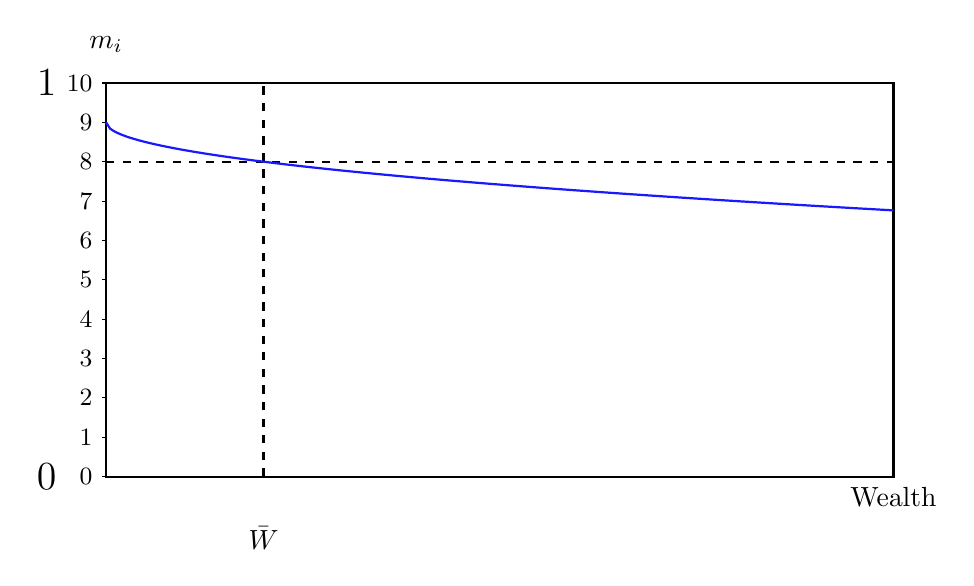
\begin{tikzpicture}[scale=.5]
% \def\bndmax{5}        %https://tex.stackexchange.com/questions/68462/filling-a-complex-region-with-tikz
% \def\bndmin{0.2}
\def\Y{10}  % height of y axis pecent
\def\W{20}  % length  of x axis
\def\Wbar{4}
\def\rbar{8}% this is the prime rate
% Equation   \[ r_i = (A + .5 \frac{\bar{W}}{W_i})\omega\]
% \def\Wmin{.63}  %This sets the lower limit fo the 
\def\Wmin{(\B*\Wbar)/(\Y/\rbar-\A)} %function to keep in in bounds
\tikzset{func/.style={thick,color=blue!90}}	
\draw [thick](\W,\Y)-- (0,\Y)node[left=.5cm]{\Large$1$}node[above=.25cm]{$m_i$} -- (0,0)node[left=.5cm]{\Large$0$}--(\W,0)node[below]{Wealth}--cycle;  	% Axes box
\draw [dashed, thick] (0,\rbar) -- (\W,\rbar);  	% Axes
\draw [thick,dashed] ( \Wbar,0)node[below=.5cm]{$\bar{W}$} -- (\Wbar,\Y);  	% Axes
\foreach \yi in {0,...,\Y} \draw (0,\yi)--(-.1,\yi)node[left]{\small$\yi$};
% \foreach \yi in {0,2,4,6,8,10} \draw (0,\yi)--(-.1,\yi));
% node[left]{\small$\yi$};
% \foreach \yi in {0,2,4,6,8,10}node at (-.1,yi) {{10*yi}} ;
\draw[func,domain=0:\W] plot [samples=200] (\x,(9-\x^.5/2);
\end{tikzpicture}
    \end{center}
    \caption{Individual borrowing ratio $m_i$ as a function of wealth}
    \label{fig-borrowing-ratio}
    \end{figure}


The borrowing ratio, $m$ is the fraction of a property's price that can be mortgaged. We assume that the bank uses a function of the form 


\begin{align}
m_i^{max\_permitted} =& \mathrm{max\_mortgage\_share} - 0.1*\left(\frac{\bar W}{ W_i}\right), \label{eqn-wealth-based-mortgage}  %^{\mathrm{wealth\_sensitivity}
\end{align} 
where $\bar{W}$ is mean wealth and $W_i$ is individual wealth.\footnote{To shift the curve  so that the curve approaches $m=0$ when $W=0$ we add  $Z=(1-m^{max})\bar W$ to the numerator and the denominator. The value is calculated by solving Equation~\ref{eqn-wealth-based-mortgage} for {$m_i^{max}=0$}.}


\subsubsection{Income-based mortgage maximum}
A common rule is that mortgage payments cannot exceed some fraction of income, $Y_i=\omega+ \psi + {r}S_i$, where $S_i$ is individual savings.
If $\mathbb{C}$ a person's carrying capacity, The annual payment that their income allows,  the capitalized value gives us an \textbf{income-based  mortgage maximum} of 


\begin{equation}
M^{max}_{Y,i} = \frac{\mathbb{C} (\omega+ \psi + {r}S_{Ni})}{r^{prime}},\label{eqn-income-based-mortgage}    
\end{equation}
% In addition, The Bank may have a maximum share of the price that it will lend, say $0.8P$. Because the actual price is unknown when buyers prequalify, this test limits the maximum bid computed below: \
% \[M^{max}i = min\left\{\frac{0.28*(\omega+w)}{r},  0.8P_0 \right\} \]
where ${r}$ is $i$'s rate of return on  $S_{Ni}=(S-M)$, the savings remaining after making the down payment,\footnote{If the constraint is binding we can  substitute $M^{max}$ for $M$and explicit function to get :
\begin{align}
M^{max}      &= 0.28 * (wage + r (S-M^{max})) / r'\nonumber\\
         &= 0.28 (wage + r (S)) / r' - 0.28 rM^{max}) / r'\nonumber\\
M^{max}(1+\frac{0.28 r}{r'}&=0.28 (wage + r S) / r'\nonumber\\
M^{max}   &=  \frac{0.28 (wage + r S )} {1+0.28 r}\nonumber   
\end{align}
} as the maximum a  buyer should pay. %\footnote{We  assume that the bank does not take transportation costs into account  when calculating income.}
%\footnote{If the expected return on a property is greater than the individual cost of borrowing, it would pay any agent to borrow as much as possible and purchase properties as they can available.}
In our model the bank uses a rule of this form to decide how much it is willing to lend to 

  \begin{figure}
    \centering
    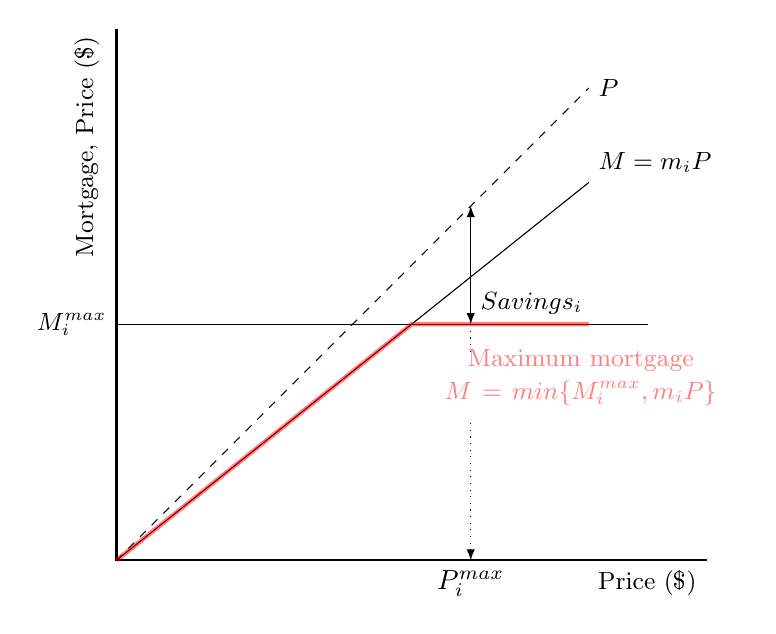
\begin{tikzpicture}	[scale=1.5]
%AXES
\draw[thick] (0,4.5) --(0,0)--(5,0)node[below left]{\small Price (\$)};
\node at (-.25, 3.5)[ rotate=90]{\small Mortgage, Price (\$)};
% M =Mi MAX
\draw[dashed] (0,0)--(4,4)node[right]{\small $P$};
\draw[] (0,2)node[left]{\small $M_i^{max}$}--(4.5,2);%node[right, red]{\small $M = M_i^{max}$};
% M =mi MAX
\draw[] (0,0)--(4,3.2)node[above right]{\small $M = m_iP$};
% COMBINED MAX RED
\draw[ultra thick, red, opacity=.5] (0,0)--(2.5,2)node[below right,  text width=4cm, align = center]{\small \\ Maximum mortgage \\ $M=min\{M_i^{max}, m_iP\}$}--(4.0,2);
% SAVINGS
\draw[latex-latex] (3,2)node[above right] {\small $Savings_i$}--(3,3);
% PMAX
\draw[dotted,latex- ] (3,0)node[below] {$P_i^{max}$}--(3,1.2);
\draw[dotted ] (3,2)--(3,1.72);
\end{tikzpicture}
    \caption{The bank's dual mortgage constraint and the savings constraint determine the maximum bid price.}
    \label{fig:dual-constraint}
    \end{figure}

\subsubsection{Combined mortgage maximum permitted by the bank for new buyers and second home buyers}

The above two equations specify two constraints on the mortgage.  Combining, we get 
\begin{align} 
M_i^{max} &= min \left\{ m_i^{max}*P, \ M^{max}_{Y,i} \right\}. 
\label{eqn-max-mortgage-combined}
\end{align}
The two constraints on mortgage size that the bank imposes are incorporated in the red line in Figure~\ref{fig:dual-constraint}. The maximum permitted mortgage is thus combined with the savings constraint to determine the maximum price that a potential home buyer can offer. The top dashed diagonal line, in Figure~{fig:dual-constraint}, is the price, $P =$ mortgage $+$ savings. The difference between the two diagonal lines is what the purchaser pays from savings. %\footnote{Equation~\ref{eqn-property-investment-return2} implies a `bang-bang' control---with all sales going to the richest participant unless there are limits on the size of capital flows. For our simulation, we implement such limits.} 
% \[M^{max}_{UY,i} = \frac{0.28*(\omega+ \psi)}{r}\] 
% It is the maximum the bank will let you pay.

% \subsection{The cost of capital}
% The cost of capital is known to differ for rich and poor. This model ties the individual cost of capital,  ${r}$ for agent $i$, to a prime rate, $\bar r$, and to individual wealth. Figure~\ref{fig-borrowing-cost} illustrates the cost of the borrowing model we implement, 
%  \[ {r} = (A + B \frac{\bar{W}}{W_i})\omega\]
% Where $\bar{W}$ is mean wealth and $W_i$ is individual wealth.   
% a kink because there are 2 constraints.  The actual mortgage must be below both lines.
% This is just the constraint. Up to the kink, little $m_i$ is a fraction of price. beyond at little $m_i$ becomes a different number - number based on little $m_i$ for everyone
% banks have an advantage since they can practically bid anything
% m - mortgage share
% P - realized price
% M - maximum - 
% \begin{figure}[!ht]
% \begin{center}
% 
% Large version
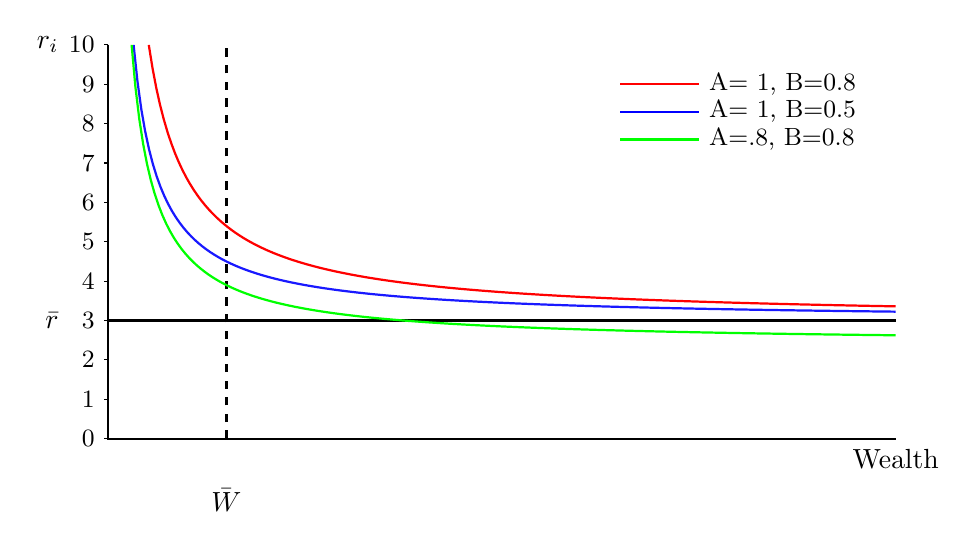
\begin{tikzpicture}[scale=.5]
%\def\bndmax{5}        %https://tex.stackexchange.com/questions/68462/filling-a-complex-region-with-tikz
%\def\bndmin{0.2}
\def \Y {10}  % height of y axis pecent
\def \W {20}  % length  of x axis
\def \Wbar {3} % jmeam wealth
\def \omega {3}
\def \A {1}  %was .5
\def \B {.5}
%Equation   \[ r_i = (A + .5 \frac{\bar{W}}{W_i})\omega\]
\def \Wmin{.63}  %This sets the lower limit fo the 
\def \Wmin{(\B*\Wbar)/(\Y/\omega-\A)} %function to keep in in bounds
	
\tikzset{func/.style={thick,color=blue!90}}	

\draw [thick] (0,\Y)node[left=.5cm]{$r_i$} -- (0,0)--(\W,0)node[below]{Wealth};  	% Axes
\draw [thick] (0,\omega)node[left=.5cm]{$\bar r$} -- (\W,\omega);  	% Axes
\draw [thick,dashed] ( \Wbar,0)node[below=.5cm]{$\bar{W}$} -- (\Wbar,\Y);  	% Axes

\foreach \yi in {0,...,\Y} \draw (0,\yi)--(-.1,\yi)node[left]{\small$\yi$};

\draw[func,domain=\Wmin:\W] plot [samples=200] (\x,{(\A+\B*\Wbar/\x)*\omega});
\def \A {.8}
\draw[func,domain=\Wmin:\W, green] plot [samples=200] (\x,{(\A+\B*\Wbar/\x)*\omega});

\def \A {1}
\def \B {.8}
\draw[func,domain=\Wmin:\W, red] plot [samples=200] (\x,{(\A+\B*\Wbar/\x)*\omega});

\draw [red,  thick](13, 9)--(15,9)node [right, black] {\small A=\ 1,\ B=0.8};
\draw [blue,  thick](13, 8.3)--(15,8.3)node [right, black] {\small A=\ 1,\ B=0.5};
\draw [green, thick](13, 7.6)--(15,7.6)node [right, black] {\small A=.8, B=0.8};
\end{tikzpicture}

% % Small version with equation and parameter values
% \[   r^h=\frac{ \delta(1+\dot p  - (1+r)m) \ + \rho   	-\kappa - t } {1-m}    \]
% \begin{tikzpicture}[scale=.35]
% %\def\bndmax{5}        %https://tex.stackexchange.com/questions/68462/filling-a-complex-region-with-tikz
% %\def\bndmin{0.2}
% \def \Y {10}  % height of y axis percent
% \def \W {18}  % length  of x axis
% \def \Wbar {3} % j mean wealth
% \def \omega {3}
% \def \A {1}  %was .5
% \def \B {.5}
% %Equation   \[ r_i = (A + .5 \frac{\bar{W}}{W_i})\omega\]
% \def \Wmin{.63}  %This sets the lower limit fo the 
% \def \Wmin{(\B*\Wbar)/(\Y/\omega-\A)} %function to keep in in bounds
	
% \tikzset{func/.style={thick,color=blue!90}}	

% \draw [thick] (0,\Y)node[left=.5cm]{$r_i$} -- (0,0)--(\W,0)node[below]{Wealth};  	% Axes
% \draw [thick] (0,\omega)node[left=.5cm]{$\bar r$} -- (\W,\omega);  	% Axes
% \draw [thick,dashed] ( \Wbar,0)node[below=.5cm]{$\bar{W}$} -- (\Wbar,\Y);  	% Axes

% \foreach \yi in {0,...,\Y} \draw (0,\yi)--(-.1,\yi)node[left]{\tiny$\yi$};

% \draw[func,domain=\Wmin:\W] plot [samples=200] (\x,{(\A+\B*\Wbar/\x)*\omega});
% \def \A {.8}
% \draw[func,domain=\Wmin:\W, green] plot [samples=200] (\x,{(\A+\B*\Wbar/\x)*\omega});

% \def \A {1}
% \def \B {.8}
% \draw[func,domain=\Wmin:\W, red] plot [samples=200] (\x,{(\A+\B*\Wbar/\x)*\omega});

% \draw [red,  thick](10, 9)--(12,9)node [right, black] {\tiny A=\ 1,\ B=0.8};
% \draw [blue,  thick](10, 8)--(12,8)node [right, black] {\tiny A=\ 1,\ B=0.5};
% \draw [green, thick](10, 7)--(12,7)node [right, black] {\tiny A=.8, B=0.8};

% \def \W {19}  % length  of x axis
% \node[right] at (\W,9.5){\small$\delta=$discount factor};
% \node[right] at (\W,8.5){\small$\dot p=$appreciation rate};
% \node[right] at (\W,7.5){\small$r=$borrowing rate};
% \node[right] at (\W,6.5){\small$m=$mortgage/price};
% \node[right] at (\W,5.5){\small$\rho=$rental  rate};
% \node[right] at (\W,4.5){\small$\kappa=$op cost rate};
% \node[right] at (\W,3.5){\small$t=$tax rate};
% \node[right] at (\W,2.5){\small$\upsilon=$use value rate};
%  \end{tikzpicture}



% One blue line with x-shift, y-shift
% \begin{figure}
% \begin{tikzpicture}[scale=.5]
% %\def\bndmax{5}        %https://tex.stackexchange.com/questions/68462/filling-a-complex-region-with-tikz
% %\def\bndmin{0.2}
% \def \Y {10}  % height of y axis pecent
% \def \W {20}  % length  of x axis
% \def \Wbar {3} % meam wealth
% \def \rbar {3}% this is the prime rate 

% %\def \Wmin{(\B*\Wbar)/(\Y/\rbar-\A)} %function to keep in in bounds
% \tikzset{func/.style={thick}}	
% 	% Axes
% \draw [thick] (0,\Y)node[left=.5cm]{$r_i$} -- (0,0)--(\W,0)node[below]{Wealth};  
% \foreach \yi in {0,...,\Y} \draw (0,\yi)--(-.1,\yi)node[left]{\small$\yi$};
% \draw [thick] (0,\rbar)node[left=.5cm]{$\bar r$} -- (\W,\rbar);  	% Axes
% \draw [thick,dashed] ( \Wbar,0)node[below=.5cm]{$\bar{W}$} -- (\Wbar,\Y);  	% 

% \def \A {1} %vertical shift aroung \rbar, the prime rate
%  \def \B {1}  % Scales the exponential curveBLUE
%  \def \C {1}  %right shift  
% % \def \Wmin {.4+\B}  %This sets the lower limit fo the 
% \def \Wmin {(\B*\Wbar)/(\Y-\rbar+\A) +\C} %function to keep in in bounds

% \draw[func,domain=\Wmin:\W, color=blue!90] plot [samples=200] (\x,{\rbar-\A+\B*\Wbar/(\x-\C))});
% \node  [align=left, text width =2cm ] at (13, 8.3) {\small y-shift=\A \newline scale=\B \newline x-shift= \C};

%  \end{tikzpicture}
% \caption{Individual borrowing cost as a function of wealth II}
% \label{fig-borrowingrate2}
% \end{figure}

% The rates $\delta,\ \sigma,$ and $r$ depend on the period, $T$. 


% LARGE WITH DIFFERENT PARAMETER VALUES THAN MAOIN FIGURE - MORE SPREAD

% \begin{figure}
% \begin{tikzpicture}[scale=.5]
% %\def\bndmax{5} % https://tex.stackexchange.com/questions/68462/filling-a-complex-region-with-tikz
% %\def\bndmin{0.2}
% \def \Y {10}    % height of y axis as a pecent
% \def \W {20}    % length  of x axis
% \def \Wbar {3}  % mean wealth
% \def \rbar {3}  % the prime rate 

% % Equation   \[ r_i = (A + .5 \frac{\bar{W}}{W_i})\omega\]
% \def \Wmin{.63}  %This sets the lower limit fo the 
% \def \Wmin{(\B*\Wbar)/(\Y/\rbar-\A)} %function to keep in in bounds
% \tikzset{func/.style={thick}}	

% % Axes
% \draw [thick] (0,\Y)node[left=.5cm]{$r_i$} -- (0,0)--(\W,0)node[below]{Wealth};  
% \foreach \yi in {0,...,\Y} \draw (0,\yi)--(-.1,\yi)node[left]{\small$\yi$};
% \draw [thick] (0,\rbar)node[left=.5cm]{$\bar r$} -- (\W,\rbar);  	% Axes
% \draw [thick,dashed] ( \Wbar,0)node[below=.5cm]{$\bar{W}$} -- (\Wbar,\Y);  	% 

% \def \A {1.0}  \def \B {0.5} %BLUE
% \draw[func,domain=\Wmin:\W, color=blue!90] plot [samples=200] (\x,{(\A+\B*\Wbar/\x)*\rbar});
% \draw [ultra thick, color=blue!70 ](13, 8.3)--(15,8.3)node [right, black] {\small A=\A,\ B=\B};

% \def \A {0.5} 
% \def \B {0.5} % GREEN
% \draw[func,domain=\Wmin:\W, color=green] plot [samples=200] (\x,{(\A+\B*\Wbar/\x)*\rbar});
% \draw [thick,  color=green](13, 7.6)--(15,7.6)node [right, black] {\small A=\A, B=\B};

% \def \A {1.0}  \def \B {0.8} % RED
% \draw[func,domain=\Wmin:\W, red] plot [samples=200] (\x,{(\A+\B*\Wbar/\x)*\rbar});
% \draw [thick,  color=red](13, 9)--(15,9)node [right, black] {\small A=\A,\ B=\B};
% % KEY
% \end{tikzpicture}
% \caption{Individual borrowing cost as a function of wealth}
% \label{fig-borrowingrate1}
% \end{figure}
% Figure of cost of borrowing
% \caption[Borrowing cost for agents depending on wealth.]{Borrowing cost for agents depending on wealth, with different values for parameters $A$ and $B$ in Equation~\ref{eqn-interest-wealth-relationship}.} %$A=1$  $B=0.5$ (blue);  $A=1$  $B=0.8$ (red), and  $A=.8$  $B=0.8$ (green).}
% \label{fig-capital-cost}
% \end{center}
% \end{figure}

\subsubsection{Individualized borrowing rates} \label{sec:borowing-rate}

    \begin{figure}
    \centering
    
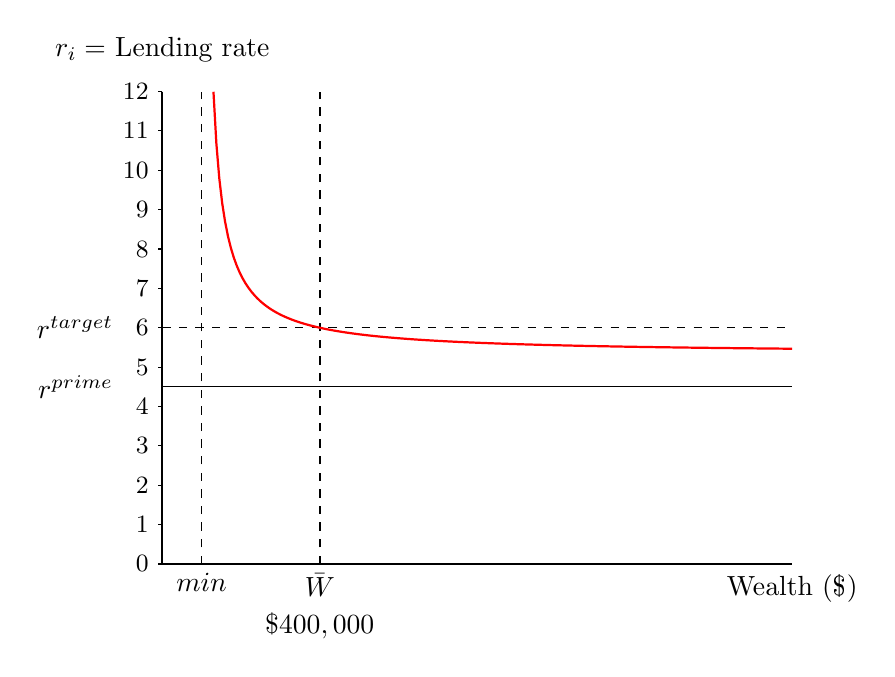
\begin{tikzpicture}[scale=.5].  %  Individual borrowing rate r\_i
%\def\bndmax{5}        %https://tex.stackexchange.com/questions/68462/filling-a-complex-region-with-tikz
%\def\bndmin{0.2}

\def \k {2}    % budget for rectangular hyperbola
\def \Wbar {4} % meam wealth in hundred thousands
\def \Wmin {1} % This sets the lower limit for lending in hundred thousands
\def \W {16}    % length  of x axis
\def \rbar {4.5} % N.B.:  this is r bar
\def \Y {12}     % height of y axis percent
\def \margin {1.5}
\def \target {\margin+\rbar} % target interest rate for bank
\def\bndmin {0.3} % This limits the function on the right so that it stays in the plotting frame
%\def \Wmin{(\B*\Wbar)/(\Y/\rbar-\A)} %function to keep in in bounds. NEEDS WORK
	
\tikzset{func/.style={thick}}	
\draw [thick] (0,\Y)node[above=.25cm]{$r_i=$ Lending rate} -- (0,0)--(\W,0)node[below]{Wealth (\$)}node[below=.5cm] {};   	% Axes

\draw [thin] (0,\rbar) node[left=.5cm]{$r^{prime}$} -- (\W, \rbar);  	% % bank rate line
\draw [thin, dashed] (0,\target) node[left=.5cm]{$r^{target}$} -- (\W, \target);  	% % target rate line
\node at ( \Wbar, 0)[below=.5cm]{$\$400,000$};  
\foreach \yi in {0,...,\Y} \draw (0,\yi)--(-.1,\yi)node[left]{\small$\yi$};  %$ put the scale on the y axis

\draw [thick, dashed] (\Wbar, 0)node[below] {$\bar{W}$} --  (\Wbar, \Y);  	%. Wbar
\draw [thin, dashed]  (\Wmin, 0)node[below] {$min$} -- (\Wmin, \Y);  %minimum lending wealth

\draw[func,domain={\W-\Wmin}:\bndmin, red] plot [samples=200] (\x+\Wmin,{\target+\k/\x - \k/(\Wbar-\Wmin)});

\end{tikzpicture}


% \begin{tikzpicture}[scale=.5]
% %\def\bndmax{5}        %https://tex.stackexchange.com/questions/68462/filling-a-complex-region-with-tikz
% %\def\bndmin{0.2}
% \def \Y {10}  % height of y axis pecent
% \def \W {20}  % length  of x axis
% \def \Wbar {4} % jmeam wealth
% \def \omega {3} % N.B.:  this is r bar

% %Equation   \[ r_i = (A + .5 \frac{\bar{W}}{W_i})\omega\]
% \def \Wmin{.63}  %This sets the lower limit fo the 
% \def \Wmin{(\B*\Wbar)/(\Y/\omega-\A)} %function to keep in in bounds
	
% \tikzset{func/.style={thick}}	

% \draw [thick] (0,\Y)node[left=.5cm]{$r_i$} -- (0,0)--(\W,0)node[below]{Wealth};  	% Axes
% \draw [thick] (0,\omega)node[left=.5cm]{$\bar r$} -- (\W,\omega);  	% Axes
% \draw [thick,dashed] ( \Wbar,0)node[below=.5cm]{$\bar{W}$} -- (\Wbar,\Y);  	% Axes

% \foreach \yi in {0,...,\Y} \draw (0,\yi)--(-.1,\yi)node[left]{\small$\yi$};

% %     ORANGE
% % \def \A {1} \def \B {.8}
% % \draw[func,domain=\Wmin:\W, orange] plot [samples=200] (\x,{(\A/\x+\B*\X/\Wbar/\x)*\omega});
% % \def \A {1} \def \B {.1}
% % \draw[func,domain=\Wmin:\W, orange, dashed] plot [samples=200] (\x,{(\A+\B*\X/\Wbar/\x)*\omega});

% %     RED
% \def \A {1} \def \B {.8}
% \draw[func,domain=\Wmin:\W, red] plot [samples=200] (\x,{(\A+\B*\Wbar/\x)*\omega});
% \def \A {1} \def \B {.1}
% \draw[func,domain=\Wmin:\W, red, dashed] plot [samples=200] (\x,{(\A+\B*\Wbar/\x)*\omega});

% %.    BLUE
% \def \A {1} \def \B {.5}
% \draw[func,domain=\Wmin:\W, blue!90] plot [samples=200] (\x,{(\A+\B*\Wbar/\x)*\omega});
% %     GREEN
% \def \A {.8} \def \B {.8}
% \draw[func,domain=\Wmin:\W, green] plot [samples=200] (\x,{(\A+\B*\Wbar/\x)*\omega});
% %.    BLACK
% \def \A {.5} \def \B {.5}
% \draw[func,domain=\Wmin:\W, black] plot [samples=200] (\x,{(\A+\B*\Wbar/\x)*\omega});


% \draw [red,  thick](13, 9)--(15,9)node [right, black] {\small A=\ 1,\ B=0.8};
% \draw [red,  thick, dashed](13, 9.7)--(15,9.7)node [right, black] {\small A=\ 1,\ B=0.1};
% \draw [blue,  thick](13, 8.3)--(15,8.3)node [right, black] {\small A=\ 1,\ B=0.5};
% \draw [green, thick](13, 7.6)--(15,7.6)node [right, black] {\small A=.8, B=0.8};
% \draw [black, thick](13, 6.9)--(15,6.9)node [right, black] {\small A=.5, B=0.5};
% \end{tikzpicture}


\label{fig-capital-cost}
    \caption{Individual borrowing rate $r_i$ price of capital}
    \label{fig:Wealth-based}
    \end{figure}

The cost of capital differs for rich and poor. We tie the individual cost of capital %,  ${r}$, for agent $i$ 
to the lender's target rate $r^{target}$, and to individual wealth. Figure~\ref{fig-capital-cost} illustrates the cost of the borrowing model we implement, which is roughly consistent with the stylized facts about lenders. 
\begin{equation}
{r} = r^{target}+ K/(W-W_{min}) -K/(\bar W - W_{min})\label{eqn-interest-wealth-relationship}
\end{equation}
for $W>W_{min}$, where  $r^{target}$ is the bank's target rate of return,  $\bar{W}$ is mean wealth and $W_i$ is individual wealth, $W_{min}$ is the level of wealth the bank requires to lend at all, and $K$ is a parameter for the wealth-sensitivity of lending. The denominator in the last two terms is simply wealth above the lender's minimum. We assume that the wealthy are lower-risk borrowers and are given preference on rates. The final term ensures that the target rate is charged for borrowers with average wealth.


%The individual cost of capital,  ${r}$ for agent $i$ is tied to a prime rate, $\bar r$ or the bank's target rate, $r^{target}$, and and varies with individual wealth. %Figures~\ref{fig-borrowing-rate1} % and ref{fig-borrowing-rate1} 
%illustrates a  possible  cost-of-borrowing models 

% \begin{align}
%  {r} =  &  \left(A + B \frac{\bar{W}}{W_i}\right) \bar r       \label{eqn-incomeandr1}  \\
%  {r} =  &  \left(\bar r - A + B *\frac{\bar W}{W_i - C}\right) \label{eqn-incomeandr2}  \\
% \end{align}
% Where $\Bar{W}$ is mean wealth and $W_i$ is individual wealth. In Equation~\ref{eqn-incomeandr2},  A determines y-shift, B, the scale, and C the  x-shift for the curve.


\subsubsection{Declining principle}\label{sec:declining-principle}

Mortgages are renewed after $\mathbb{T}$ years. During that period some of the principle has been paid off. This is most important when a property is sold. The seller gets $P-M_{i,\mathbb{T}}$, where  $M_{i,\mathbb{T}}$ is its remaining mortgage.

% % {\color{red} 

% **** ADD BACK
% \textbf{Footnote on size of mortgage at renewal.}
% % \footnote{We would need to calculate the decline balance when  renewal came up to know what assets a person has. We need a function that gives us the size of the mortgage remaining at each renewal or at the time of sale, $M_{i,term}$, for each subsequent renewal. The  function depends on the mortgage renewal term, $\mathbb $, the number of terms $term$  that have passed since the purchase, the interest rate ${r}$ and the payment. Mortgages are usually intended to be paid off over, say,  $L=25$ years If we use $T=5$, there will be 4 renewals and the house will b =e paid off at the end of the fifth. Payments are larger than the interest, so the amount owed at the end of each month declines. At the end of month N it is

% % There is a standard formula for choosing the payment so that the mortgage it is paid off at the end of the mortgage life, $L$. Say $n$ is the number of monthly payments (for example 25*12=300) %https://en.wikipedia.org/wiki/Mortgage_calculator

% % \[payment= {r}^\mathbb{\mathbb{T}}M \left[\frac{(1+{r}^\mathbb{T}\mathbb{T})^n}{(1+{r}^\mathbb{T})^n-1} \right]\]
% % Where ${r}^\mathbb{T}$ is the interest rate compounded for $\mathbb{T}$ periods.
% % % \begin{align}
% % % M_{N*T}&=(1+r)^{N}M_0-p_{N}c\nonumber \\
% % % &{}=(1+r)^{N}P-{\frac {(1+r)^{N}-1}{(1+r)-1}}c \nonumber\\
% % % &{}=(1+r)^{N}P-{\frac {(1+r)^{N}-1}{r}}c
% % % \end{align}
% % % Amount owed at end of month N}
% % %}
% % }
% % }

% \textbf{We can assume is paid off the mortgage when we discuss retirement decisions. If as person works 40 years and buys a house by the 15th year they will have paid off their  mortgage and collect the entire price if they sell. }  

% When else will we need to consider this problem? If we let people buy a revenue property - then wealth includes $P-M$. Also if we let people die early, or allow them to change homes part way through a career- for family reasons.


\subsection{Bid price}\label{sec:bid-price}
A bidding process determines the realized market price, with bidders taking into account potential capital gains. In this section, we describe the formation of the maximum bid price that we use in the bidding model. The maximum \gls{bid price}, $P_{B,ij}^{max}$ %, where i and j refer to the individual and the property involved,\footnote{We suppress the $ij$ identifiers for the rest of this chapter. }  
is the value of a property to the owner or to a potential buyer. It will differ across individuals depending on their cost of capital, discount rates,  savings, and access to mortgage funding. The same equation used to calculate the bid price used to compute the \gls{reservation price}, the minimum price that an owner will sell a property for. 

The model distinguishes between two types of investment buyers, institutional buyers and homeowners buying an investment home. They use the same investment formula, but may have different values of the parameters determining their bid prices.

We first calculate the net present value of the purchase, then divide by the amount of capital employed, which we assume is simply the size of the down payment made at the beginning of the period. This gives us a rate of return.\footnote{An alternative approach would be to calculate an \gls{internal rate of return} (IRR), but the IRR is in general the solution to a polynomial and does not guarantee a single-valued result \cite{robinsonOptimalTerminationIRR1996}. Multiple real-valued  IRRs may arise;  complex-valued IRRs may arise;  the IRR is, in general, incompatible with the \gls{net present value} (NPV) in accept/reject decisions; the IRR ranking is, in general, different from the NPV ranking; the IRR criterion is not applicable with variable costs of capital. Ways to salvage the IRR as a usable criterion have been proposed that are consistent with our approach \cite{magniAverageInternalRate2010}.} The rate of return on the investment must exceed some required rate of return. This condition allows us to calculate the maximum bid that will satisfy that criterion.}
% We assume that agent may be  speculating on potential \glspl{capital gain} as well as on the \gls{use value} or net market rent they get from the property. We therefore treat the purchase as an investment decision and compute a rate of return, $v$, conditional on the price paid. This allows us to 
We then solve this for the maximum bid, $P_{max}^{bid}$ that achieves the desired rate of return. 


% The underlying value of a home is the capitalized value of the services it provides, which are perpetual.  Rents, however, depend on urban productivity and may change over time. Any expected increase in future rents capitalized into the market price of a home as a capital gain for the owner. Home prices should respond to expectations.

% As Horowitz \cite{horowitzBiddingModelsHousing1986} notes, a prospective buyer considering a vector of attributes of the property, including the seller's asking price and the property taxes, transaction costs, and financing costs at a specified price. The  potential buyer also is likely to have estimates of the maintenance costs and resale value of the house, although these may be highly subjective. All of these factors shape whether an investment is profitable. To make a comparison with alternative investments, it is necessary to compute a rate of return.

The agent who purchases makes a down payment, $D$ on a house for a price, $P_0$, and agrees to pay off a mortgage, $M$ with interest at the end of the mortgage period.  The purchaser  receives the increased price 
$P_T = (1 + \dot P)^\mathbb{T}P_0 =(1+\dot P_\mathbb{T})P_0 $, 
after a period $\mathbb{T}$, Where $\dot P$  is the expected annual rate of price increase and we define $\dot P^\mathbb{T}$
or $\dot P^{^\mathbb{T}}$ 
as the $\mathbb{T}$-period  price-growth rate. The agent also receives either the net market rental value of the property throughout the period, $\mathcal{R}_N$, or if the owner is also the resident, the locational rents. 
 
% With a price-growth rate of $\dot P$ per year, the growth over $T$ years is $(1+\dot P)^\mathbb{T}$, and  %and a 5 year mortgage period, 
% the expected price at the end of the period is:

% \[P_M^{Te}=P_0(1+\dot P)^\mathbb{T}\]

% If, for example price growth is 10\%, $\dot P= 0.1$, the {capital gain}, or growth, over a 5-year mortgage term is 0.61051 $\approx$ 60\% of the original price, $P_0$.

%The expected rate of price growth, $P_{M_j}^\epsilon$, is an estimate based on rents and past market behaviour. In our computational model we employ a regression model to generate an \gls{expected market price} based on past prices. The rate of price growth $\dot P$ we use in our model of investor behaviour is derived from the same regression model.




% TODO SOME REFERENCES - what are these? MOVE? \cite{anselinModernSpatialEconometrics2014, gelmanDataAnalysisUsing2006}.


 
\subsubsection{Rent and mortgage costs}
Both mortgage payments and net rent revenue can be calculated as sum of regular payments, each of which accumulates interest to the end of the mortgage period. This is called a ``uniform series compound amount.'' \cite{sullivanEngineeringEconomy2003} For net rent at the end of the mortgage renewal term we write
\begin{equation}
\mathcal{R}_{N, \mathbb{T}}= \frac{(1+r)\mathbb{^\mathbb{T}}-1}{r}\mathcal{R}_N.     
\end{equation}

The regular mortgage payment for each period is $rM=rmP_0$.\footnote{We assume that the regular payment covers only the interest and that the full mortgage is due at the end of the period.} Using the same calculation, the value of the mortgage payments is 
\begin{equation}
\mathcal{M}_{\mathbb{T}} = \frac{(1+r)^\mathbb{T}-1}{r}rmP_0. 
\end{equation}
Both these amounts are discounted by $\delta^\mathbb{T}$ to the present. % in our calculation.
 
\subsection{The value of an investment with price growth or interest}
 The model in this section is central to our agents' housing purchase decisions. It incorporates individual access to capital and capital costs, expected capital gains and property revenues.  
 
 For an agent, the value $V$ of a property investment over  $\mathbb{T}$ years is the capital gain, $P_{^\mathbb{T}}-P_{0}$, minus financing costs, plus net rent. % revenues.
% \[\mathcal{R}_{N, \mathbb{T}}=  \delta^\mathbb{T}\frac{(1+r)^\mathbb{T}-1}{r}\mathcal{R}_N  \]
% To keep the notation simple, let 
% \[\delta_r^\mathbb{T}=\delta^\mathbb{T}\frac{(1+r)^\mathbb{T}-1}{r}\]
% The present value of the mortgage repayment plus the accumulated interest be 
% \[\bar M^\mathbb{T}_r = \delta^\mathbb{T}\frac{(1+r)^\mathbb{T}-1}{r}\]
 We can write $V$ in terms of the purchase price, and several individual parameters: interest rate, share of the price that can be mortgaged and discount rate %\footnote{The down payment could be deducted in advance, but if the discount rate is equal to the interest rate it drops out completely.}
 
 \begin{align}
V &= \delta^\mathbb{T}\left( P_\mathbb{T}-P_0-\mathcal{M}_{\mathbb{T}}- M+ \mathcal{R}_{N, \mathbb{T}} \right)      \nonumber\\
&= \delta^\mathbb{T}\left( P_\mathbb{T}-P_0- \left(\frac{(1+r)^\mathbb{T}-1}{r}rmP_0\right)- M+ \mathcal{R}_{N, \mathbb{T}} \right)      \nonumber\\
&= \delta^\mathbb{T} \left(
\dot P_\mathbb{T} P_0 -\left((1+r)^\mathbb{T}-1\right)mP_0-mP_0
 +  \mathcal{R}_{N, \mathbb{T}} \right) 
%\label{first_sub}\nonumber
\\
  &= \delta^\mathbb{T} \left((\dot P_\mathbb{T} - (1+r)^\mathbb{T}m) P_0 + \mathcal{R}_{N, \mathbb{T}}\right),\label{eqn_investment_value}
\end{align}
where $\dot P_\mathbb{T}=\frac{P_\mathbb{T}-P_0 }{P_0}$  is the expected  change in the market price over the term of the mortgage as a fraction of the original price.
$V$ is the net present value of buying and selling after one mortgage renewal period of $\mathbb{T}$ years. %All rates are scaled to the length of the period to avoid the need for compounding calculations. 
% The function has four individualized parameters, $\delta$, $\dot p$, $r$, $m$. %, as well as any factors that affect the rent or other terms.


\subsubsection{Rate of return on investment}
We divide $V$ by the size of the down payment, $D=P_0-mP0$, to get the  rate of return  

\begin{align}
r^{return} =
  &= \frac{V}{D}  \nonumber \\
  &= \delta^\mathbb{T} \left((\dot P_\mathbb{T} - (1+r)^\mathbb{T})m \frac{P_0}{D} + \frac{\mathcal{R}_{N, \mathbb{T}}}{D}\right) \nonumber \\
%  &= \delta^\mathbb{T} \left((\dot P_\mathbb{T} - (1+r)^\mathbb{T})m \frac{P_0}{P_0-mP_0} + \frac{\delta_r^\mathbb{T}\mathcal{R}_{N, \mathbb{T}}}{P_0-mP_0}\right)\\
   &= \delta^\mathbb{T} \left((\dot P_\mathbb{T} - (1+r)^\mathbb{T})m \frac{P_0}{P_0-mP_0} + \frac{\mathcal{R}_{N, \mathbb{T}}}{P_0-mP_0}\right) \nonumber \\
  &= \frac{\delta^\mathbb{T}}{1-m} \left((\dot P_\mathbb{T} - (1+r)^\mathbb{T})m  + \frac{\mathcal{R}_{N, \mathbb{T}}}{P_0}\right).\label{eqn-property-investment-return1} 
\end{align}
Notice that the return depends on the price paid, $P_0$, which is determined in the market though competitive bidding.

\subsubsection{Capital gains tax}
The \gls{capital gains tax} is %one of the most interesting policy parameters to consider. It is 
a tax on the increase in value of a property that results form an increase in the price. The capital gains tax is a tax on speculative return on housing as an investment. In our model captures some or all of the expected gain from rising locational rents. We can introduce it in Equation~\ref{eqn-property-investment-return1} by multiplying $\dot P_\mathbb{T}$ by 1 minus the capital gains tax rate, representing the share of the capital gains that a buyer is permitted to keep. We allow the rate for occupant owners to differ from the rate for non-occupant owners.


\subsection{Criterion for investment}
Equation~\ref{eqn-property-investment-return1} provides a criterion for investors. %\footnote{Section~\ref{sec-extensions-conversion}, in Appendix~\ref{appendix-future-work}, discusses the potential for more detailed modelling of the land assembly and development process.} 
 Agents invest if  their expected return is greater than the target return they are seeking:
\begin{equation}
r^{target}\le r^{return} 
\label{eqn-property-investment-return2}
\end{equation}
For the bank R target is the prime rate plus a margin. For individuals it woulds be the the best alternative investment they have. It can be argued that  $r^{target}_i$ should be the long-term bond rate. We provisionally set $r^{target}_i=r^{prime}$.

\subsubsection{Maximum bid for investors}
Equation~\ref{eqn-property-investment-return2} combined with the rate of return calculation in Equation~\ref{eqn-property-investment-return1} are used to calculate a maximum bid price for investors for use in the bargaining model.
% Equation~\ref{eqn-return-on-investment} makes it clear that the estimated rate of return depends on subjective magnitudes,$\delta$ and $\dot P_M^e$, attributes of the property, $ \mathcal{R}_N$, and  individual financial position, $r$, $m$.
% 
%Buyers will not initially bid the maximum and sellers will generally set an asking price $P^{ask}$ higher than their reservation price $P_R$, so we build a simple bargaining process.
Buyers and sellers calculate the maximum amount they are willing to pay for a property.  Investors are not concerned with amenities, while residents are. %Since investors are concerned with the rent they can collect, however
Amenities enter through the net rent term for investors, to the extent that residents are willing to pay for amenity. Buyers differ in having individualized values for $r$, $\delta$, $m$, and $M$.%To simplify notation, we continue to omit  $i$ subscripts for each of these terms
\footnote{Transaction costs on the sale are omitted. They are actually large. We can easily add a term to  Equation~\ref{eqn:maximum-bid} to examine the effect of transaction costs.} % on the distribution of wealth.}

\begin{align}
r^{target}& \le \frac{\delta^\mathbb{T}}{1-m} \left((\dot P_\mathbb{T} - (1+r)^\mathbb{T})m  + \frac{\mathcal{R}_{N, \mathbb{T}}}{P_B^{max}}\right)\nonumber\\
\frac{(1-m)}{\delta^\mathbb{T}}r^{target} &\le \dot P_\mathbb{T} - (1+r)^\mathbb{T}m  +   \frac{\mathcal{R}_{N, \mathbb{T}}}{P_B^{max}} \nonumber\\
\frac{(1-m)r^{target}}{\delta^\mathbb{T}} - \dot P_\mathbb{T} + (1+r)^\mathbb{T}m &\le  \frac{\mathcal{R}_{N, \mathbb{T}}}{P_B^{max}}\nonumber\\
P_B^{max} &\le  \frac{\mathcal{R}_{N, \mathbb{T}}}{(1-m)r^{target}/\delta^\mathbb{T} - \dot P_\mathbb{T} + (1+r)^\mathbb{T}m}. \label{eqn:maximum-bid}
\end{align}
We call this  $i's$ maximum bid.\footnote{The denominator in Equation~\ref{eqn:maximum-bid} can be seen as an adjusted rate of return for capitalizing net rents, analogous to the value of $r$ in the standard capitalization formula.} 
It represents the maximum a buyer is willing to pay, the value of the stream of rent plus any capital gains. % It is also the most reasonable reservation price.%\footnote{In principle Equation~\ref{eqn:maximum-bid} could be calculated for all potential buyers and sellers for every property. In practice, only a subset of potential buyers and sellers are in the market at any time.} 
If the buyer intends to become a resident, the net rent term Equation~\ref{eqn:maximum-bid} is replaced by a housing-services-and-amenity term, which represents non-monetary income. % and is another form of locational rent. 

\subsubsection{A simple proxy for $\dot P_\mathbb{T}$}

The \gls{market price} or the price at which a property is exchanged on the market, $P_M$ will not be known in advance, nor will the future sale price.  In order to make decisions, agent $i$ must form an \glspl{expectation} or prediction $P_{M_i}^{\epsilon}$ of the as yet unrealized future market price. Case and Shiller observe that, ``People seem to form their expectations from past price movements rather than having any knowledge of fundamentals. \cite{caseThereBubbleHousing2003}. They further argue that the 1-year expectations are fairly well described as attenuated versions of lagged actual 1-year price changes. Our $\dot P_\mathbb{T}$ is a forecast or expectation by agents in the model of the change in price over a period $\mathbb{T}$.

Since our version of the \gls{Alonzo model} implies that house prices will rise by the capitalized value of an increase in the wage premium, a rational investor might use a forecast of the wage premium to develop a long-term forecast of house prices, and from that of $\dot P_\mathbb{T}$. %The specific value to use for $\die{\omega}{t}$ might depend on assumptions agents make about adjustment,  the variability of $P$, and the observability of $\omega$, but 
We will assume that agents simply observe the the most recent change in $\omega$  correctly and expect it to persist.\footnote{In principle, agents might form an expectation by observing past prices for each class of home. To mimic this process we could compute average price changes per period at each distance from the centre and use them to form a forecast for the mortgage period $\mathbb{T}$. }

In Equation~\ref{eqn_investment_value} we defined $\dot P$ as $\frac{P_\mathbb{T}-P_0}{P_0} $, where $\mathbb{T}$ indicates the. end of the mortgage period. $P_0$ is the warranted price, 
\[P_W =\frac{1}{r}\left[\omega - {dc} + \mathbb{A} + a\psi\nonumber  + a*b*\psi\right]\]
Only the wage premium changes in this analysis. A change in the wage premium that is expected to be permanent results in a change in the warranted price:  \[\die{P_W}{t} = \frac{1}{r}\die{\omega_t}{t}.\]
If we assume that the price will continue to change at the same rate over the mortgage term, the change is compounded, and we write

%P_W &=\frac{1}{r}\left[\omega - {dc} + \mathbb{A} + a\psi\nonumber  + a*b*\psi\right] \nonumber\\

%Only $\omega$ is expected to change over time, so  
%Since \[\dot P= \frac{\die{P_W}{t}}{P_T} \]


\begin{align}
\dot P  &= \frac{1}{r}\left[\left(\frac{\omega_t-\omega_0}{\omega_0}+1 \right)^\mathbb{T}-1\right], \nonumber\\
        &=\frac{1}{r}\left[\left(\frac{\omega_t}{\omega_0} \right)^\mathbb{T}-1\right]. \nonumber
\end{align}



\subsection{Illustrating constraints on the bid price} \label{sec:bids-and-reservation}
 
Buyers calculate their maximum bid based on value, but actual bids are constrained by the mortgage limits imposed by the bank illustrated in Figure~\ref{fig:dual-constraint} and the buyer's savings. The mortgage constraint may or may not bind, depending on the price of the final price. Figure~\ref{fig:savings-constraint} illustrates how these considerations affect the actual bid. 

We choose a price on the horizontal axis and project it up to the black dashed diagonal. Three lines show the levels of the constraints at that price.
% {\color{red}
%Purchasers may be financially constrained by the combination of mortgage availability and savings, as illustrated in Figure~\ref{fig:savings-constraint}. 
\begin{enumerate}
    \item The horizontal dashed line $P_B^{max}$ represents \textbf{the maximum the buyer is willing to pay}, as calculated in Equation~\ref{eqn:maximum-bid}, if the mortgage funding were available. No bid will be above this line. 

    \item The kinked thick red line combines the three conditions on the size of the mortgage imposed by the bank based on wealth and income and on the bank's equity requirement.
   
    \item The thick blue line, $min\left\{m_i P,\  M_{i}^{max}\right\}+ S $, represents the purchaser's combined financial constraints, determined by mortgage availability and savings. It is \textbf{the maximum the buyer is able to pay}.  No bid will be above this line either.
\end{enumerate}
 As a result the combined curve will be the constraint for buyers, and the requirement that the bid be below both the blue and black lines can be written

\begin{equation}
    Constrained\; P_{B} \le min \left\{P^{max}_B, min\left\{m_i P,\  M_{i}^{max}\right\}+ S \right\}.  \label{eqn:bid_diagonal}
\end{equation}

% \begin{align}
%     constrained\; P_B^{max} &\le min\left\{ P_B^{max} ,  \frac{M^{max}}{m} , \frac{S}{1-m}  \right\} \label{eqn:maximum-bid-restricted}
% \end{align}
% where $A^{net}$ is the net  amenity gain.



 \begin{figure}
    \centering
    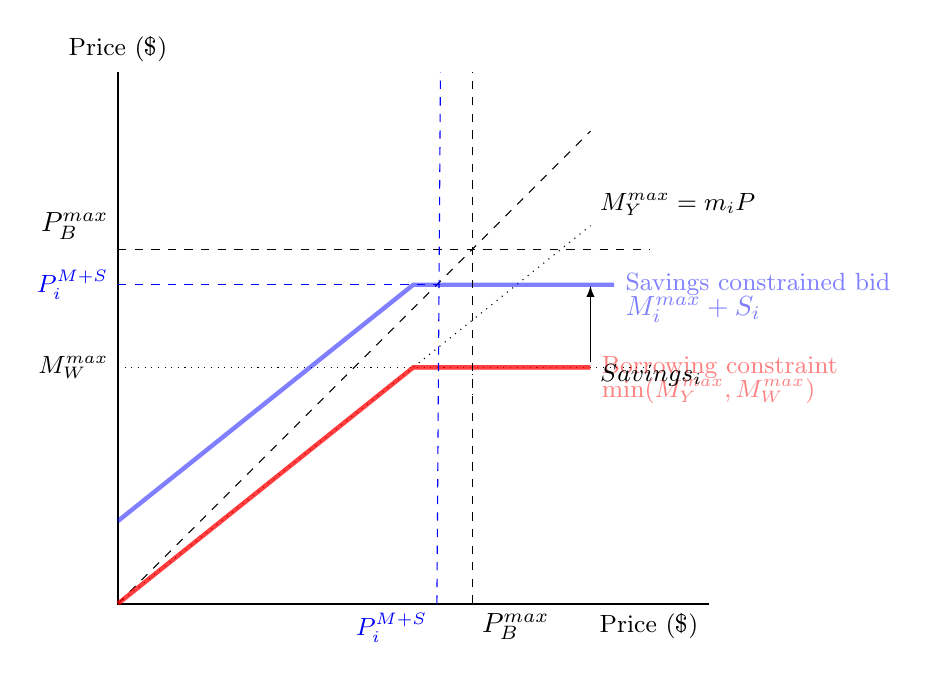
\begin{tikzpicture}	[scale=1.5]
%AXES
\draw[thick] (0,4.5)node[above]{\small Price (\$)} --(0,0)--(5,0)node[below left]{\small Price (\$)};
%\node at (-.25, 3.5)[ rotate=90]{\small Mortgage, Price (\$)};
% M =Mi MAX
\draw[dashed] (0,0)--(4,4);{node[right]}; %{\small $P$};
\draw[dotted] (0,2)node[left]{\small $M_W^{max}$}--(4.5,2);%node[right, red]{\small $M = M_i^{max}$};
% M =mi MAX
%\draw[dotted,red, opacity=.5] (0,0)--(4,3.6)node[right]{\small $M = 0.9P$};
\draw[dotted] (0,0)--(4,3.2)node[above right]{\small $M^{max}_Y = m_iP$};
% COMBINED MAX RED
\draw[ultra thick, red, opacity=.5] (0,0)--(2.5,2)--(4.0,2)node[right]{\small Borrowing constraint};
\draw[ultra thick, red, opacity=.5] (0,0)--(2.5,2)--(4.0,2)node[below right]{\small min($M_{Y}^{max},M_{W}^{max}$) };

\draw[ultra thick, blue, opacity=.5] (0,.7)--(2.5,2.7)--(4.2,2.7)node[right, ]{\small Savings constrained bid}node[below right, ]{$M_i^{max}+S_i$};
% SAVINGS
\draw[-latex] (4,2.05)node[below=5, right] {\small $Savings_i$}--(4,2.69);
% PMAX
\draw[dashed, ] (3,0)node[below right] {$P_B^{max}$}--(3,4.5);%node[, right]{\small desired max bid};
\draw[dashed,] (0,3)node[above left] {$P_B^{max}$}--(4.5,3);%node[, right]{\small desired max bid};

\draw[dashed, blue, thin] (2.7,0)node[below left] {\small $P_i^{M+S}$}--(2.73,4.5); %node[left, text width= 2cm]; %{\small };
\draw[blue, thin, dashed] (0,2.7)node[left] {\small $P_i^{M+S}$}--(2.73,2.7);%node[left, text width= 2cm]{\small savings constrained bid};
\draw[dotted ] (3,2)--(3,1.72);
\end{tikzpicture}
    \caption{Desired bid  and savings + mortgage constrained bid}
    \label{fig:savings-constraint}
    % I removed a line saying Savings sub i in lower corner
    \end{figure}

%
%If you are on the sloped line, constrained by $m$, the price is

% my version
% \begin{equation}
%     P_{B} \le min\Big(  min(m_i P_{B,i}^{max},\ M^{max}_i)+ S_i,\  P_{B,i}^{max}\Big)
% \end{equation}


% HOW DO WE COMPUTE DELTA? 
% \begin{lstlisting}
%     def get_discount_factor(self):
%         """
        
%         The discount factor gives the present value of one dollar received at particular point in the future, given the date of receipt and the discount rate.
%         Delta is the subjective individual discount rate for agent
%         after one year. This will be close to the prime interest rate, r_i.
%         """  
%         self.r_discount= .07
%         delta = 1/ self.r_discount
%         delta_period_1 = 1 / (1 + r_discount) 
%         delta_mortgage_period = delta_period_1**self.mortgage_period
%         #sum_delta = (1 - delta_mortgage_period)/delta
%         #return sum_delta
%         # sum_delta = delta_mortgage_period * (1 - delta_mortgage_period)
% \end{lstlisting}

\subsection{The bargaining model} \label{sec:bargaining-model}
Buyers place bids and a sale occurs if there is a surplus created by the transaction, that is if the the buyer's maximum bid exceeds owner's \gls{reservation price}, the maximum the owner would pay to retain their own property. 
Bargaining models attempt to identify the way the surplus available from a transaction is divided between the parties involved. Possible divisions are described by the red line in Figure~\ref{fig:Nash-bargaining-game}.\footnote{The classic  formulation by John Nash %\cite{Nash_John% (1953-01-01). "Two-Person Cooperative Games". Econometrica. 21 (1): 128–140. doi:10.2307/1906951. JSTOR 1906951, The Nash equilibrium: A perspective. Charles A. Holt and Alvin E. RothAuthors Info & Affiliations March 15, 2004 101 (12) 3999-4002 https://doi.org/10.1073/pnas.0308738101} 
identifies  `\gls{disagreement point},' which which is the  lowest value each player will accept. The combination of reservation price and maximum bid together are the disagreement point for a two-person price bargaining game. Since paying for the house is a negative for the buyer, the scale on the vertical axis  in Figure~\ref{fig:Nash-bargaining-game} is reversed to generate a version of the most common Nash bargaining figure.} 

    \begin{figure}
        \centering
        
  \begin{tikzpicture}[scale=1]
%  \draw [gray, opacity=.7] (0,0) grid (7,7);
\draw [<->] (0,6) node[above]{$buyer$}-- (0,0)node[left]{0}node[below]{0} -- (6,0) node[below]{$Seller$};
\draw [red, thick ] (1,7)--(7,1);
\draw [red, line width=1mm] (3,5)--(5,3);
\draw [red, thick, fill= yellow, opacity=.5] (3,3)--(3,5) -- (5,3)--cycle;

% vertical
\draw [blue, dashed] (0,5)node[left]{50,000}--(5,5)node[below right]{will not pay more}--(5,0)node[below]{50,000};
\draw [blue, ] (0,3)node[left]{30,000}--(6,3)node[above right]{can not get more};
% Horizontal
%\draw [blue, dashed] (4,0)--(4,6)node[above right]{will not accept less};
\draw [blue, ] (3,0)node[below]{30,000}--(3,6)node[above right]{can not offer less};
%\draw [ ultra thick] (0,0)--(1.5,1.5)node[ right]{equal set};
%\draw [dashed] (1,1) --(2,1)-- (2,0);
%\draw [red, ultra thick, dashed] (0,0) --(2.4,1.2)node[above]{relative equal set};
%\node at (2,1)[below right, ]{$(max\ u_1,\ max\ u_2)$};
%\node at (3.5,3){Agreement set};\node at (3,3.5){\Large A};

\node at (3,3)[below left, text width=2.8cm, align=right]{\textbf{disagreement\newline point}};
\node[mark size=4pt,color=red] at (3,3) {\pgfuseplotmark{square*}};

\end {tikzpicture}


        \caption{The Nash bargaining game}
        \label{fig:Nash-bargaining-game}
    \end{figure}


In Figure~\ref{fig:Nash-bargaining-game} we imagine the seller values the property at \$30,000 (the reservation price) and the buyer values it at \$50,000 (the maximum bid price).  At any price above \$30,000 the seller is better off. At any price below \$50,000 (above -\$50,000 on the vertical axis) the buyer is better off. 
The set of acceptable bargains acceptable to both is above and to the right of the point labeled `disagreement point.' 

In principle the buyer could pay more than \$50,000 or the seller could accept a price below \$30,000, but neither would do so if they are rational. 
The thick red line segment, called the bargaining set, represents all the outcomes that are\begin{enumerate}
    \item Efficient, because the entire \$20,000 surplus is allocated to the players. 
    \item Feasible, because the players involved gain no more in total than the potential increase in value generated by the transaction.
    \item Rational because neither player has to accept an outcome that makes them worse off.
\end{enumerate}   

The bargaining processes will ideally lead to a point on that thick red line segment. In practice, some of the surplus is dissipated in the sale process, and some is absorbed by intermediaries. We ignore this refinement for the current version of the model. Differences in relative power will tip the outcome in favour of the stronger player.   Players who can afford to wait will get a larger share of the gain. Excess demand favours sellers. Low vacancy rates favour owners over tenants.   If there is a deal, it will still be at a price between the maximum bid and the reservation price, and in most cases probably somewhere near the midpoint. Sellers might reduce the asking price if the home fails to sell in the first period it is on the market.\footnote{Uncertainty adds further complications. Parties may not know each other's disagreement point. PartieS post asking prices greater than their reservation price or initial offers much lower than their true valuation.  
Negotiations often proceed through a series of offers and counteroffers.}\;\footnote{In an overheated housing market bid prices might exceed asking prices, but the price won't exceed the maximum expected profitable bid price, $P_B^{max*}$. We could elaborate the model by defining a measure of \gls{sellers' bargaining power} based on vacancies and expected prices.}   % Ariel Rubinstein \cite{rubinsteinPerfectEquilibriumBargaining1982} presented a convincing solution to the alternating offers model in a 1982 paper. His process converges to the Nash solution. 
% }
%  The higher asking price and lower bids are `cheap talk' (In game theory, cheap talk is communication between players that does not directly affect the payoffs of the game. % This is in contrast to signaling in which sending certain messages may be =


 


% \subsubsection{Maximum bids}
% The rate of return calculation in  Equation~\ref{eqn-property-investment-return1} combined with the investment criterion in Equation~\ref{eqn-property-investment-return2} identifies the maximum  that price that an investor can price offer for a property  and still maker sa profit.

% \begin{align}
% %r^{target}& \le \frac{\delta^\mathbb{T}}{1-m} \left(\dot P_\mathbb{T} - (1+r)^\mathbb{T})m  + \frac{\mathcal{R}_{N, \mathbb{T}}}{P_B^{max}}\right)\nonumber\\
% % (1-m)r^{target}/\delta^\mathbb{T} &\le \dot P_\mathbb{T} - (1+r)^\mathbb{T}m  +   \frac{\mathcal{R}_{N, \mathbb{T}}}{P_B^{max}} \\
% % (1-m)r^{target}/\delta^\mathbb{T} - \dot P_\mathbb{T} + (1+r)^\mathbb{T}m &\le  \frac{\mathcal{R}_{N, \mathbb{T}}}{P_B^{max}}\nonumber\\
% P_B^{max} &\le  \frac{\mathcal{R}_{N, \mathbb{T}}}{(1-m)r^{target}/\delta^\mathbb{T} - \dot P_\mathbb{T} + (1+r)^\mathbb{T}m} \label{eqn:maximum-bid}
% \end{align}

% We call this  $i's$ maximum bid.
% .\footnote{The denominator in Equation~\ref{eqn:maximum-bid} can be seen as an adjusted rate of return for capitalizing net rents, analogous to the value of $r$ in  the standard capitalization formula.} 
% It represents the value of the stream of rent plus any capital gains, and is therefore the most reasonable reservation price for sellers as well the most reasonable maximum offer for potential buyers. In principle it exists for all potential buyers and sellers for every property. In practice, only a subset of potential buyers and sellers are in the market at any time. 




\subsubsection{The many-to-one matching problem}
\textbf{The housing market is usually a many-to-many matching problem}: which property goes to which buyer? For each property that comes on the market, there will be a set of potential buyers with differing maximum bids. Some simplifications are available. In each sale, the bidder with the highest bid price among those currently bidding on that property will make the purchase.\footnote{For many reasons the process is likely to exhibit a good deal of randomness and inefficiency. For our purpose, the general messiness of the market is unlikely to do more than slow and blur results somewhat.} Since the highest bidder is competing with the second-highest bidder, we expect the final price to be equal to the second-highest maximum bid, shown as the star in figure~\ref{fig:auction-game}. 


    \begin{figure}
        \centering
        
\begin{tikzpicture}[scale=1]
%  \draw [gray, opacity=.7] (0,0) grid (7,7);
\draw [<->] (0,8.25) node[left, text width=1cm]{Buyer pays}-- (0,0)node[left]{0}node[below]{0} -- (8.25,0) node[below right, text width=1cm]{Seller gets};
\draw [red, thick, latex-latex ](1.5,5.5)node[below left, black, text width=1cm]{Feasible\\ set}-- (2,6)--(6.5,1.5)--(6,1);
\draw [red, line width=1mm] (3,5)--(5,3);
\draw [red, thick, fill= yellow, opacity=.5] (3,3)--(3,5) -- (5,3)--cycle;

% % vertical axis
\draw [dashed] (0,5) node[left] {-\$30,000} -- (3,5) ;
\draw [dashed] (0,3) node[left] {-\$50,000} -- (5.5,3) ;
\draw [dashed] (3,0) node[below]{ \$30,000} -- (3,5.5) ;
\draw [dashed] (5,0) node[below]{ \$50,000} -- (5,3) ;
\draw [dashed, thick, blue] (0,2) node[left] {-\$60,000} -- (7,2)
node [right,text width=2cm]{highest bid};

%  \draw[pattern=north west lines, distance=2mm,pattern color=red!30, draw=none] (0,0) rectangle (3,8);
%  \node[text width=2.5cm] at (1.5,7) {\small Seller will not accept less than \$30,000};

% \draw[pattern=north east lines, pattern color=green!60, draw=none] (0,0) rectangle (9,3);
% \node[text width=2.5cm]at (7,1.5)  {\small Buyer will not pay more than \$50,000};

\draw [ latex-latex, ultra thick](3.7,7)-- (3,7)--(3,3)--(7,3)node[right,text width=2cm]{second highest bid}--(7,3.7)node[above ]{Rational Set} ;
\draw [ latex-, thick, red](3.5,4.5)-- (4,5)--(5.5,5)node[right]{Bargaining Set} ;

\draw [ latex-, thick, red](2.5,5.5)-- (3.6,6.5)--(5.5,6.5)node[right]{Efficient Set} ;%name

%\draw [ latex-, thick, red](3.5,4.5)-- (4,5)--(5.5,5)node[right]{Bargaining Set} ;

%\draw [dashed] (1,1) --(2,1)-- (2,0);
%\draw [red, ultra thick,3 dashed] (0,0) --(2.4,1.2)node[above]{relative equal set};
%\node at (2,1)[below right, ]{$(max\ u_1,\ max\ u_2)$};
%\node at (3.5,3){Agreement set};\node at (3,3.5){\Large A};

\node at (3,3)[left, text width=1.8cm, align=right]{\textbf{\tiny Disagreement\newline point}};

\node[mark size=4pt,color=red] at (3,3) 
{\pgfuseplotmark{square*}};

\node[mark size=8pt,color=blue] at (5,3) 
{\pgfuseplotmark{10-pointed star}};

\draw;
\end {tikzpicture}
        \caption{Auction with a second, higher bid}
        \label{fig:auction-game}
    \end{figure}

%.\footnote{We could allow potential buyers  to approach potential sellers who have not listed with an offer and allow worker-owners to consider retiring early or becoming tenants if an offer is attractive.  This is only likely if speculative pressures are strong. It may require having multiple institutional buyers to make offers more competitive. In that case, initial offers will be closer to the maximum bid price, tending to pull prices up and benefit potential sellers.}  
When there is one bidder, we will employ a simple rule for splitting the gain from trade. Both simplifications are grounded in standard bargaining theory.

 
    \begin{figure}[!thb]
    \centering
    \begin{tikzpicture}
%\draw[step=0.5cm,color=gray] (0,-3) grid (8,7);
\node [above](Bank)at (1,7) {Bank};
\node [above](Buyers)at (5,7) {Buyers $i$};
\node [above](Seller)at (7,7) {Seller};

\draw[ultra thick, -latex](Bank)--++(0,-1.5)node[below]{$P_B^{max}$};
\draw[ultra thick, -latex](Buyers)--++(0,-1.5)node[below]{$P_i^{max}$};
\draw[ultra thick, blue!60,-latex](Seller)--++(0,-1.5)node[below]{$P_R$};

\node[above, red, text width=1.55cm, align=center]at (3,5){Select two highest bids};

\begin{scope}[shift={(0,-1)}]
\draw[ultra thick](1,6.)--(5,6.0); % Bar
\draw[ultra thick, blue!60,-latex](7,6.2)--++(0,-1)--++(-4,0)node[left, red]{Compare};  %Pass P_R to if-then
\draw[ultra thick, -latex](3,6)--++(0,-1.5)--++(-2.,-.5);% down and left
\draw[ultra thick, -latex](3,5)--++(0,-1)node[below, text width=1.5cm, align=center]{none above {$P_R$} };%
\draw[ultra thick, -latex](3,5)--++(0,-.5)--++(2.2,-.5)node[below, text width=1.cm, align=center]{One above {$P_R$} };
% down and Right

\draw[ultra thick, -latex](.1,2.5)node[above, text width=2.cm, align=center]{two or more above {$P_R$} }--++(0,-.75)node[below, text width=3cm, align=center]{Auction: price is second highest $P_i^{max}$, house goes to highest bidder};

\draw[ultra thick, -latex](3,2.5)--++(0,-.75)node[below, text width=2cm, align=center]{No sale};

\draw[ultra thick, -latex](5.5,2.5)--++(0,-.75)node[below, text width=2cm, align=center]{Bargain: price is power-modified mean};
\end{scope}

\end{tikzpicture}
    \caption{The Bargaining model and price determination}
    \label{fig:Bargaining}
    \end{figure}



\subsubsection{The bargaining process}
We have now identified a set of bids and a reservation price for each property on the market that must be converted to a price for that property using the bargaining rule. 
The bargaining  mechanism then simply has to compare the maximum bid price $P_B$ with the seller's reservation price. If the $P_B^{max}>P_R$, a deal that is between the two values is possible. Otherwise, the transaction does not proceed.
If a bargain is possible, the rule is simple: 
\begin{enumerate}
    \item If there is only one maximum bid above the reservation price, split the difference between the bid and the reservation price evenly.\footnote{It is fairly simple if perhaps not very revealing to incorporate relative power. % as described in Footnote~\ref{fn:relative-power}.
    }
    If $P_B^{max}>P_R$,  the bargaining rule selects a value 
    \[P = xP_B^{max}+(1-x)P_R, \ \ \ x\in [0\dots 1] \]
where $x$ is typically 0.5.
    \item If there are two or more maximum bids above the reservation price, the property goes to the highest and since the bids are the maximum the buyers would pay under any circumstances, the price is set a the second highest bid in order to reflect the tightness of the market.\footnote{This is an application of Vickrey \gls{second-price auction} theory\cite{levinAuctionTheory2004}.} 

\end{enumerate}
 
% \[P^{ask}>P_M^e> 0.95 P^r\]
% Otherwise
% \[P^{ask}> 1.10P^r>P_M^e\]
% If no offer exceeds the reservation price, no sale is made.

% Once an owner reached retirement age, if no sale is made the reservation price is reduced for the next cycle.
% If no sale is made the owner considers becoming a landlord. if the present value of net rent is above the reservation price, the owner rents out the home. 



\section{Linking financialization and urban productivity}


% {\color{red}We model a relationship between productivity and agglomeration. }


As we point out in Chapter~\ref{chapter-tramsmission} there are numerous channels through which financialization might affect the productivity of the city. The available literature does not tell us which channels are active, if any, and which of those have a significant effect. Our goal in modelling is to establish whether or not linkages would have significant effects on the economy. If our model establishes that the effects are potentially significant, it might encourage researchers to explore this neglected area in urban economics.


The channels we discussed in  Chapter~\ref{chapter-tramsmission}  all have their influence on the Alonzo-Jacobs cycle in our model, either through a reduction in the inputs to production, labour and capital, or by changing parameters  $A$, $\alpha$, $\beta$, or $\gamma$ of the production function. It is likely to be difficult to disentangle influences on the parameters empirically. Their effects on productivity are all positive. They are each likely to have several components, including common components, and measurement at the level of a city would involve aggregating many firms in many industries.     

In the class of models we draw on, the scale parameter $A$ controls the overall productivity. It might captures several productivity-enhancing effects: the contribution of urban infrastructure (including transportation infrastructure), technology, ownership ratios, participation by residents, local investment in productive capital, regulatory structure, the presence of local universities, the skill level of the supporting workforce, the complexity of supply chains, or other factors. None of these are explicit inputs in our model in the way technology is in some of the growth literature described in Chapter~\ref{chapter-growth}.\footnote{Public inputs like the transportation system do not appear directly any of the models.} 
Missing explanatory variables are likely to inflate the residuals in estimates of $A$.

To introduce the potential effect of financialization and ownership as simply as possible, we rewrite $A$ from the basic model ``as:\[ A= A_0 + effectiveness*share * rent*\]
where $A_0$ represents outside or general factors contributing to productivity, $0<effectiveness<1$ is how much the local share of rents matters, and  $share*rent$ stands for the share of the urban locational rents captured by residents and contributing to local productivity. That there are local factors is indicated by the variability of estimates of $A$ in empirical studies.\footnote{See Chapter~\ref{chapter-tramsmission} Subsection~\ref{sec-fig-residuals} for references and an illustration.} 
The share term is itself a composite of the actual land-ownership share of residents determined by the housing market and the propensity to invest locally.

 
\section{Chapter summary}
In this chapter we developed  the  rules that agents in the our agent-based model follow. In doing this we have defined variables and institutional features, and developed a description of the bargaining process behind all of the adjustments. The formulae developed here are implemented in the python simulation model. Details of the adjustment speeds and parameter setting are not discussed here because they have to be `tuned'. The parameter space of the model is large, and cities only exist in a sub-region of the space. For example, if the marginal product of labour is too low, cities cannot exist. If it is too high the city explodes. We have identified a region with plausible values in which city behaviour corresponds to what we know about the evolution of cities. 

The relationships set out in this chapter are theoretically grounded and  realistic. They allow us to implement the three sub-models described in the introduction to this thesis in code. The resulting simulation model lets us demonstrate some implications of standard urban economic theory that were plausible a-priori, but that have not been formally demonstrated before.  
